\subsection{Gradient Descent Analysis}
    First we looked at our library of gradient descent methods to figure out what and how they worked. This with the goal of finding a descent recipe for optimising our neural networks down the line.
    
    \subsubsection{OLS Optimisation}
        All plots regarding the optimisation of the OLS cost function are found in \cref{res:fig:lrates}. The best MSE scores and learning rates are tabulated in \cref{res:tab:OLS_MSEs}. We found that the none of the algorithms come really close to the analytical OLS solution, found by matrix inversion, with a validation MSE of $0.1176$. The best performing algorithms were SGD with Adam (MSE $0.1660 \pm 0.0018$), SGD with momentum (MSE $0.1729 \pm 0.0022$) and GD with momentum (MSE $0.1775 \pm 0.0026$).

        In \cref{res:fig:lrate1} we see that both the non-stochastic and stochastic algorithms performed better when momentum was added, which helped avoid local minima to converge faster and prevent exploding gradients. Generally, the stochastic algorithms had tighter confidence intervals, signalling that they are not as sensitive to the initial conditions as the plain algorithms.

        Exploring the increase in epochs and decrease in batch size in \cref{res:fig:lrate2}, we see that decreasing batch size made the algorithm less stable, and more easily prone to exploding gradients. Increasing the number of epochs improved the result, and made increased the convergence, but did not affect stability.

        Adding the tuning of the learning rate with AdaGrad, we see in \cref{res:fig:lrate3} a marked increase in stability. However, the algorithms struggled to converge, with the momentum based algorithms doing best; SGD slightly bettering the GD results. However, even AdaGrad SGD with momentum could not beat the ordinary momentum based GD and SGD algorithms.

        Introducing RMSprop and Adam to tune the learning rate provided algorithms with a tunable learning rate that converged faster than AdaGrad, seen in \cref{res:fig:lrate4}. Instead of exploding, the MSE of RMSprop gradually increased from around $\eta=0.1$. Ultimately, it performed similarly to the AdaGrad algorithms, with an optimal MSE of 0.1863. The momentum based Adam algorithm performed the best, with an optimal MSE of $0.1660$; but performing well from very low $\eta$-values up to around $\eta=0.35$. After this point Adam was markedly less stable than the AdaGrad algorithms. Aside from converging faster, it was also notable that both RMSprop and Adam were much less sensitive to initial conditions, with generally much tighter confidence intervals.

        \cref{res:fig:GD_history} shows how GD with momentum, plain SGD, SGD with momentum and Adam SGD converged by epoch. The non-stochastic method converged smoothly, and was very stable. Adding stochasticity clearly exhibited unstable convergence, but overall trended downwards faster. Notably, SGD with momentum was quite explosive, whereas Adam managed to implement stochasticity and momentum in a much more stable way.

        \begin{table}[!ht]
            \centering
            \begin{tabular}{r|c|l}
                Method & MSE & $\eta$ \\ \hline
                Analytic & 0.1377 & - \\
                Plain GD & $0.1982 \pm 0.0061$ & 0.072 \\
                Momentum GD & $0.1775 \pm 0.0026$ & 0.13 \\
                Plain SGD & $0.1862 \pm 0.0028$ & 0.069 \\
                Momentum SGD & $0.1729 \pm 0.0022$ & 0.12 \\
                AdaGrad GD & $0.2135 \pm 0.012$ & 0.50 \\
                AdaGrad Momentum GD & $0.1836 \pm 0.0024$ & 0.52 \\
                AdaGrad SGD & $0.1906 \pm 0.0038$ & 0.50 \\
                AdaGrad Momentum SGD & $0.1822 \pm 0.0020$ & 0.47 \\
                RMSprop SGD & $0.1859 \pm 0.0027$ & 0.019 \\
                Adam SGD & $0.1660 \pm 0.0018$& 0.32 \\
            \end{tabular}
            \caption{Table of the best validation MSE scores by GD algorithm, together with the learning rate that produced the best result.}
            \label[tab]{res:tab:OLS_MSEs}
        \end{table}

        \begin{figure}[ht!]
            \centering
            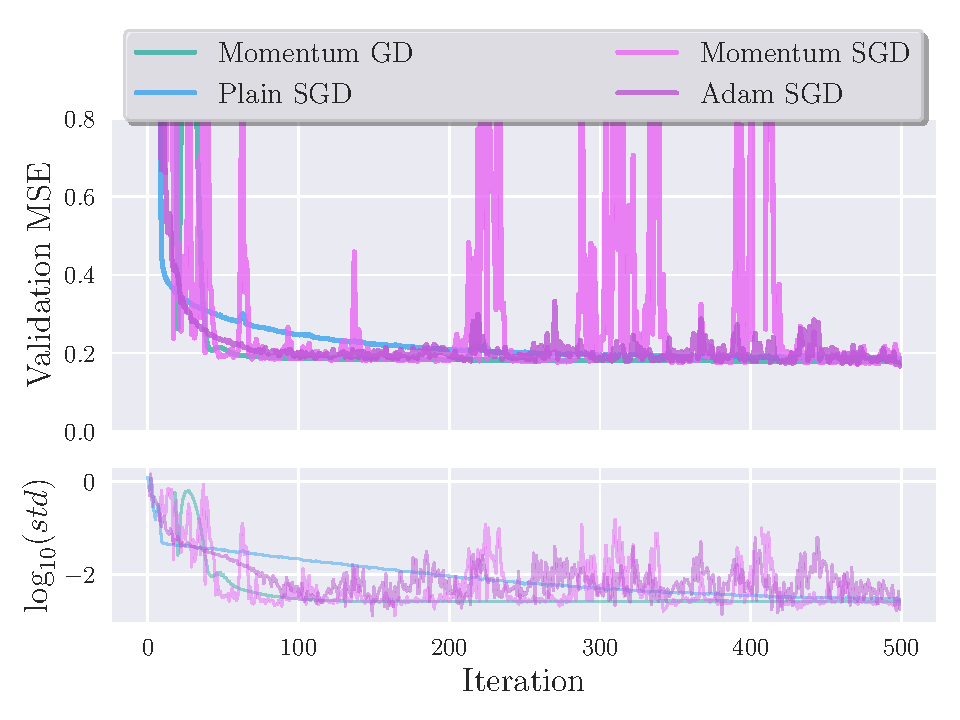
\includegraphics[width=\linewidth]{figs/GD_history.pdf} 
            \caption{Plot of the mean validation MSE of four a linear regression on Franke function data as optimised with GD algorithms after every epoch up to 500. Underneath, the logarithm of the std of the mean across descent from 5 starting points is shown. The momentum methods used $\gamma=0.8$, Adam had $\beta_1=0.9, \beta_2=0.99$ and the stochastic methods all used a batch size 200.\\
            Best MSEs were: GD w/momentum (0.1775 in iteration 500), Plain SGD (0.1862 in iteration 495), SGD w/momentum (0.1729 in iteration 486), SGD Adam (0.1660 in iteration 500).}
            \label{res:fig:GD_history}           
        \end{figure}

        \begin{figure*}
            \begin{subfigure}{.49\textwidth}
                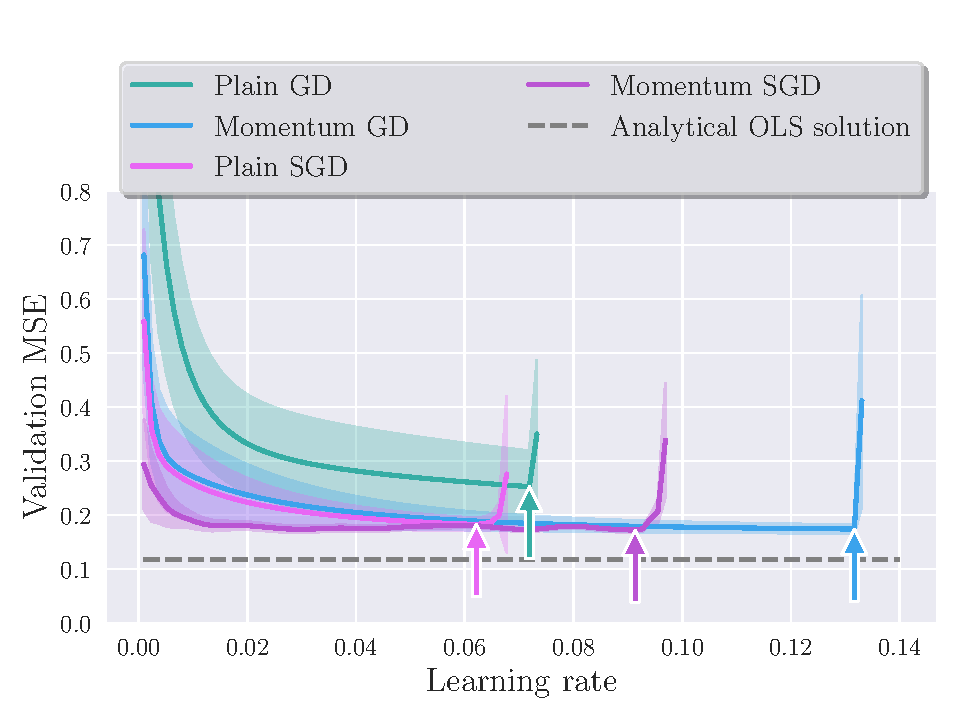
\includegraphics[width=\linewidth]{learning_rates_PGD_MGD_PSGD_MSGD.pdf}
                \caption{The minimal MSEs by algorithm: plain GD 0.1982 ($\eta=0.072$), GD w/momentum 0.1775 ($\eta=0.13$), plain SGD 0.1862 ($\eta=0.069$), SGD w/momentum 0.1729 ($\eta=0.12$)}
                \label[fig]{res:fig:lrate1}
            \end{subfigure}
            \hfill
            \begin{subfigure}{.49\textwidth}
                \centering
                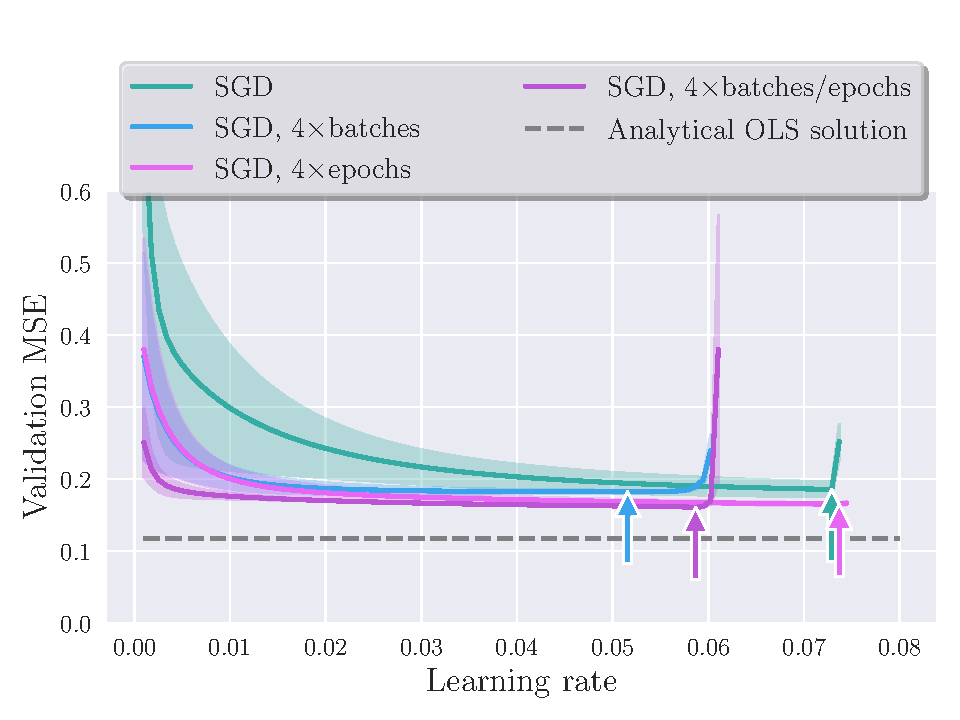
\includegraphics[width=\linewidth]{learning_rates_SGD_batches_epochs.pdf}
                \caption{The minimal MSEs of plain SGD by number of epochs and batch size: 500 epochs/200 batch size 0.1862 ($\eta=0.068$), 500 epochs/50 batch size 0.1819 ($\eta=0.0026$), 2000 epochs/64 batch size 0.1776 ($\eta=0.071$), 2000 epochs/50 batch size 0.1773 ($\eta=0.057$)}
                \label[fig]{res:fig:lrate2}
            \end{subfigure}
            \hfill
            \begin{subfigure}{.49\textwidth}
                \centering
                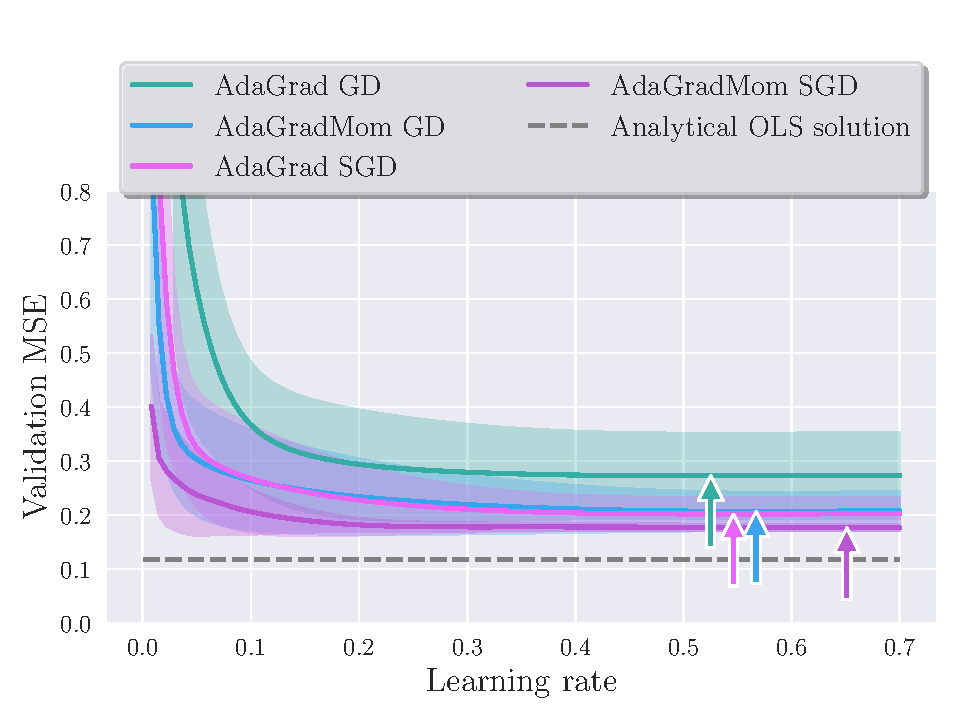
\includegraphics[width=\linewidth]{learning_rates_adagrad}
                \caption{The minimal MSEs by algorithm: AdaGrad GD 0.2135 ($\eta=0.50$), AdaGrad GD w/momentum 0.1836 ($\eta=0.52$), AdaGrad SGD 0.1906 ($\eta=0.50$), AdaGrad SGD w/momentum 0.1822 ($\eta=0.47$)}
                \label[fig]{res:fig:lrate3}
            \end{subfigure}
            \hfill
            \begin{subfigure}{.49\textwidth}
                \centering
                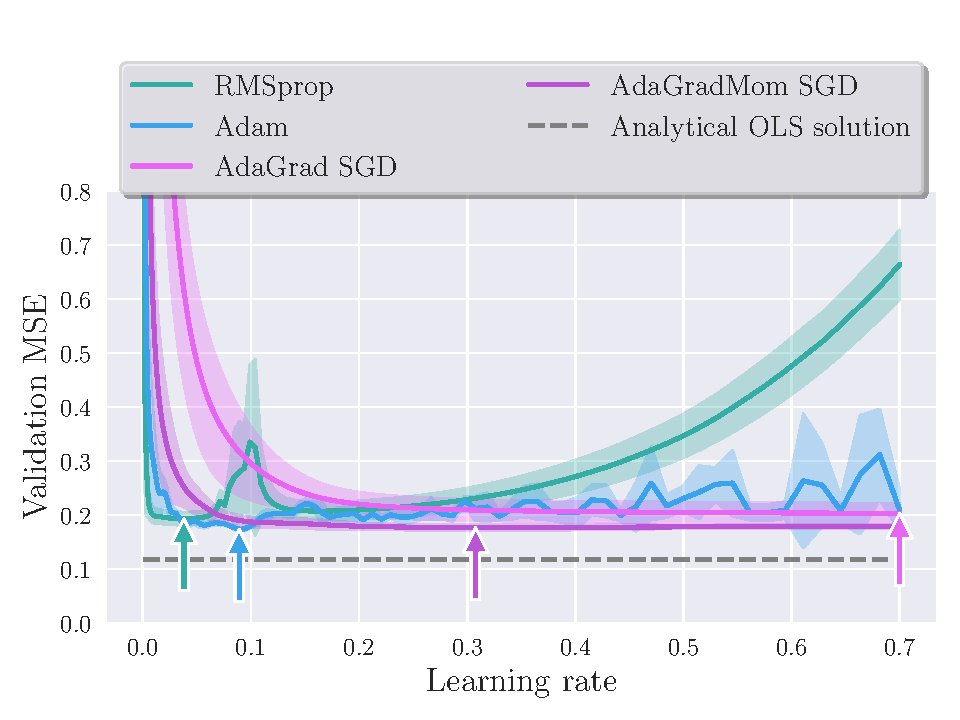
\includegraphics[width=\linewidth]{learning_rates_tunable}
                \caption{The minimal MSEs by algorithm: RMSprop SGD 0.1859 ($\eta=0.019$), Adam SGD 0.1660 ($\eta=0.32$), AdaGrad SGD 0.1906 ($\eta=0.50$), AdaGrad SGD w/momentum 0.1823 ($\eta=0.46$)}
                \label[fig]{res:fig:lrate4}
            \end{subfigure}
            \caption{Plots of the validation MSE of the parameters found from optimising the OLS cost function on Franke function data with $n=600$ data points with a train test split of $\sfrac{3}{4}$. For the momentum methods we used $\gamma=0.8$, for RMSprop we used $\beta=0.9$ and for Adam we used $\beta_1=0.9, \beta_2=0.99$. The stochastic methods used a batch size of 200 and 500 epochs, while the standard GD did 500 iterations unless specified otherwise. Overlaid are 95\% confidence intervals based on optimising with five different starting points. Exploded gradients are clipped out of the plot. The analytical OLS solution achieved an MSE of 0.1377.}
            \label[fig]{res:fig:lrates}
        \end{figure*}

    \subsubsection{Ridge Optimisation}
        The results from the ridge analysis are found in \cref{res:fig:GDridge}, and a summary is tabulated in \cref{res:tab:ridge_MSEs}. 
        
        We did not see much change in the performance of the algorithms from the OLS optimisation. There was in fact a slight decrease in the optimal MSE of all the algorithms except AdaGrad with momentum, however, the std of the MSEs generally went down. There was no universal $\lambda$-value that gave the best results. It is worth noting that there was little effect on where the exploding gradients occur; in fact with larger $\lambda$-values they occur earlier for both GD and SGD with momentum.

        The best performing algorithm was again SGD with Adam to tune the learning rate (MSE of $0.1673 \pm 0.0020$), as before with the OLS cost function.

        To see whether ridge actually had the potential to do a difference, we plotted the validation MSE of the analytical ridge solution as a function $\lambda$ against the analytical OLS solution in \cref{res:fig:ridge_ana}. We see that the ridge solution does actually perform better than OLS between $\lambda \in [0.0001, 0.01]$, meaning that there is potential for improvement with the ridge penalisation.

        \begin{table}[ht!]
            \centering
            \scalebox{0.85}{
            \begin{tabular}{r|c|l|l}
                Method & MSE & $\eta$ & $\lambda$ \\ \hline
                Analytic & 0.1338 & - & 0.002 \\
                Momentum GD & $0.1777 \pm 0.0025$ & 0.13 & $10^{-4}$ \\
                Momentum SGD & $0.1747 \pm 0.0020$ & 0.12 & $10^{-8}$ \\
                AdaGrad Momentum SGD & $0.1822 \pm 0.0013$ & 0.48 & $10^{-3}$ \\
                Adam SGD & $0.1673 \pm 0.0020$ & 0.32 & $10^{-5}$
            \end{tabular}
            }
            \caption{Summary of the best validation MSEs resulting from the optimisation of the ridge cost function using various GD algorithms. The data is taken from the plots in \cref{res:fig:GDridge}.}
            \label[tab]{res:tab:ridge_MSEs}
        \end{table}

        \begin{figure*}
            \begin{subfigure}{.49\textwidth}
                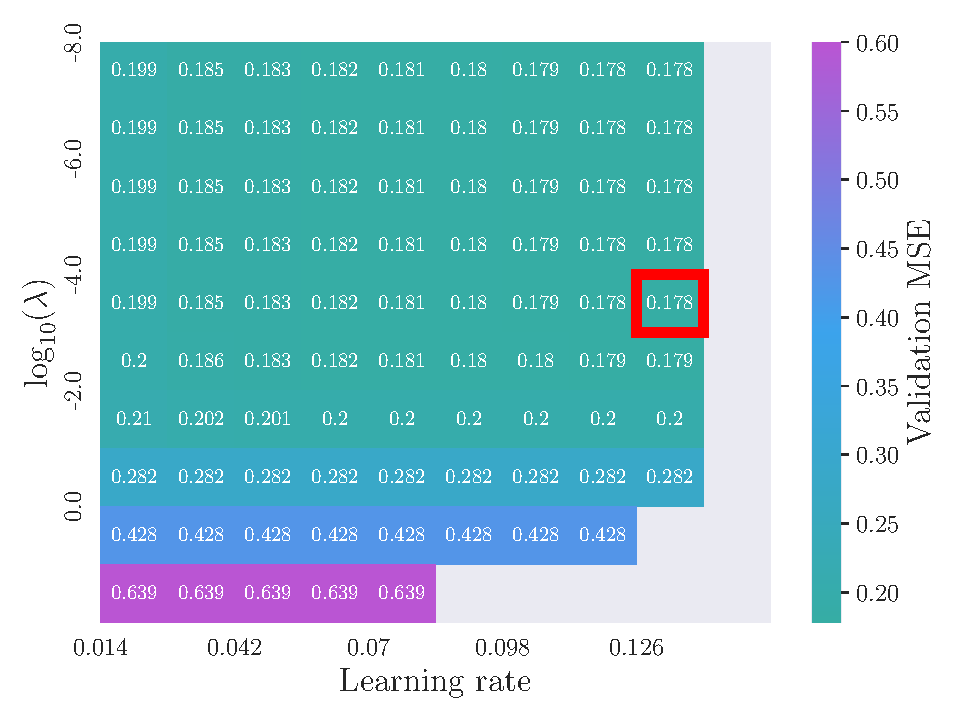
\includegraphics[width=\linewidth]{lmbda_learning_rates_momentum_GD.pdf}
                \caption{\textbf{GD with momentum}. Best MSE value was 0.1777 with $\lambda=10^{-4}, \eta=0.13$.}
                \label[fig]{res:fig:mGDridge}
            \end{subfigure}
            \hfill
            \begin{subfigure}{.49\textwidth}
                \centering
                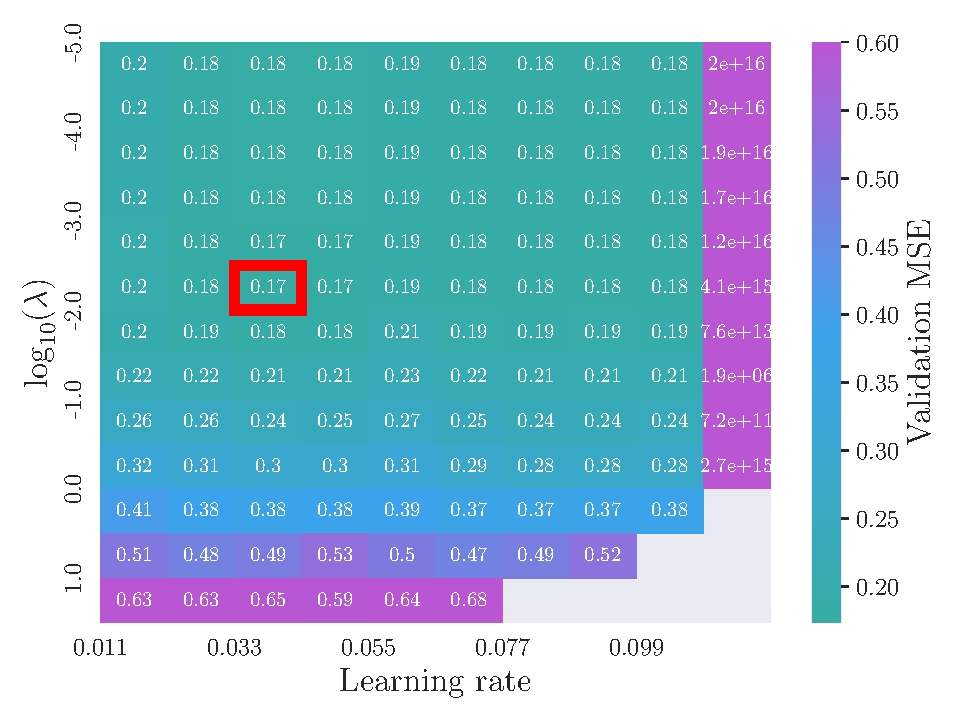
\includegraphics[width=\linewidth]{lmbda_learning_rates_momentum_SGD.pdf}
                \caption{\textbf{SGD with momentum}. Best MSE value was 0.1747 with $\lambda=10^{-8}, \eta=0.12$.}
                \label[fig]{res:fig:mSGDridge}
            \end{subfigure}
            \hfill
            \begin{subfigure}{.49\textwidth}
                \centering
                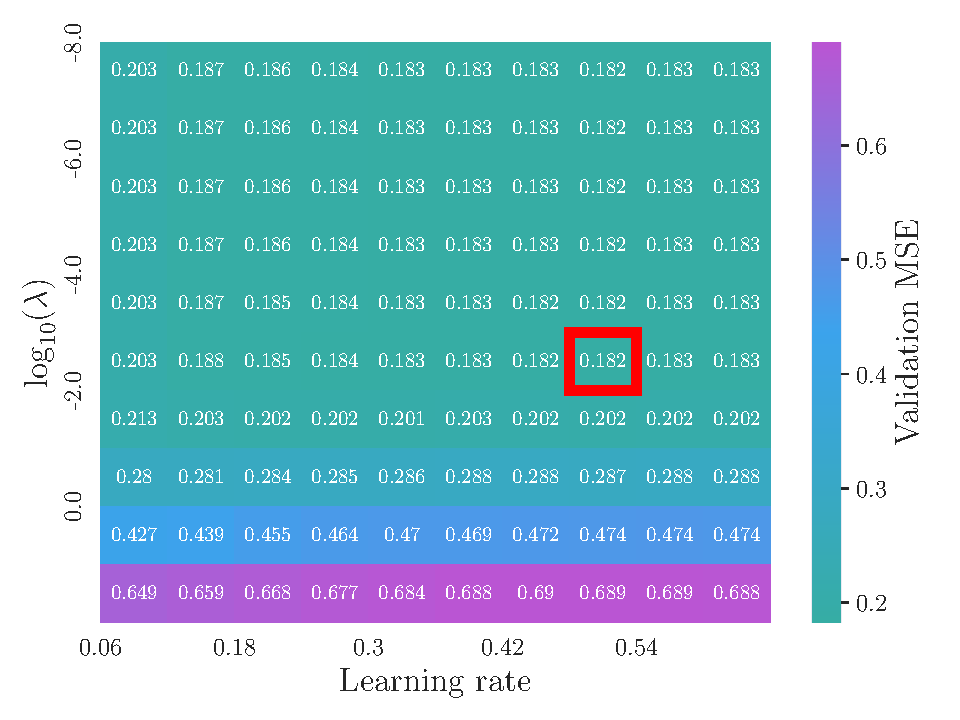
\includegraphics[width=\linewidth]{lmbda_learning_rates_adagrad_momentum_SGD.pdf}
                \caption{\textbf{SGD AdaGrad with momentum}. Best MSE value was 0.1822 with $\lambda=10^{-3}, \eta=0.48$.}
                \label[fig]{res:fig:agSGDridge}
            \end{subfigure}
            \hfill
            \begin{subfigure}{.49\textwidth}
                \centering
                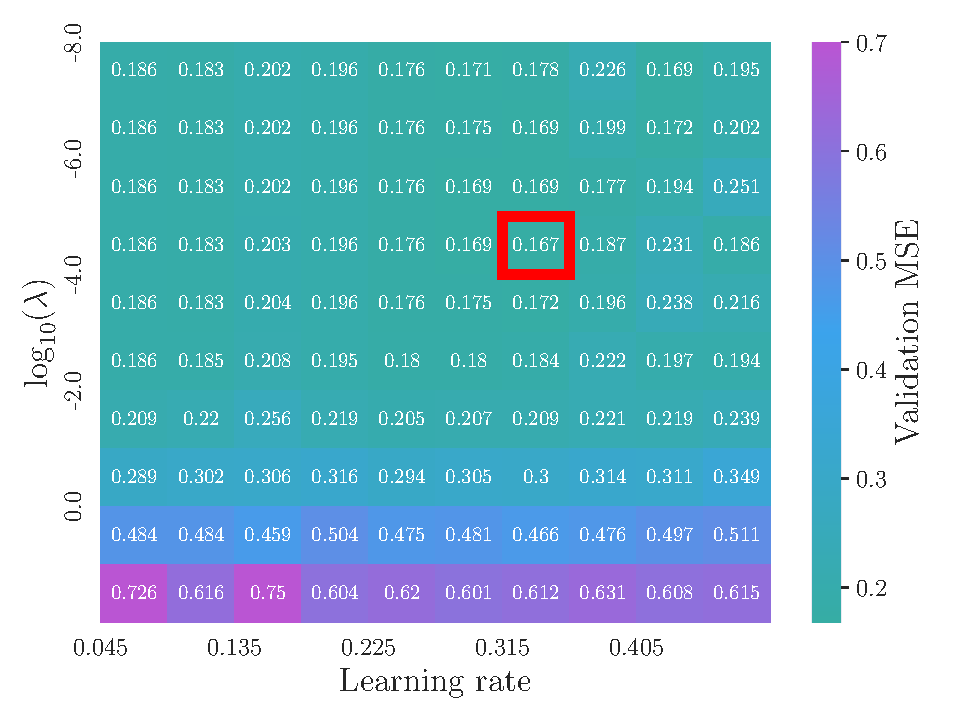
\includegraphics[width=\linewidth]{lmbda_learning_rates_adam_SGD.pdf}
                \caption{\textbf{SGD Adam}. Best MSE value was 0.1673 with $\lambda=10^{-5}, \eta=0.32$.}
                \label[fig]{res:fig:adSGDridge}
            \end{subfigure}
            \caption{Plots of the validation MSE of the parameters found from optimising the ridge cost function on Franke function data with $n=600$ data points with a train test split of $\sfrac{3}{4}$. For the momentum methods we used $\gamma=0.8$ and for Adam we used $\beta_1=0.9, \beta_2=0.99$. The stochastic methods used a batch size of 200 and 500 epochs, while the standard GD did 500 iterations unless specified otherwise. Overlaid are 95\% confidence intervals based on optimising with five different starting points. Exploded gradients are clipped out of the plot.}
            \label[fig]{res:fig:GDridge}
        \end{figure*}

        \begin{figure}[ht!]
            \centering
            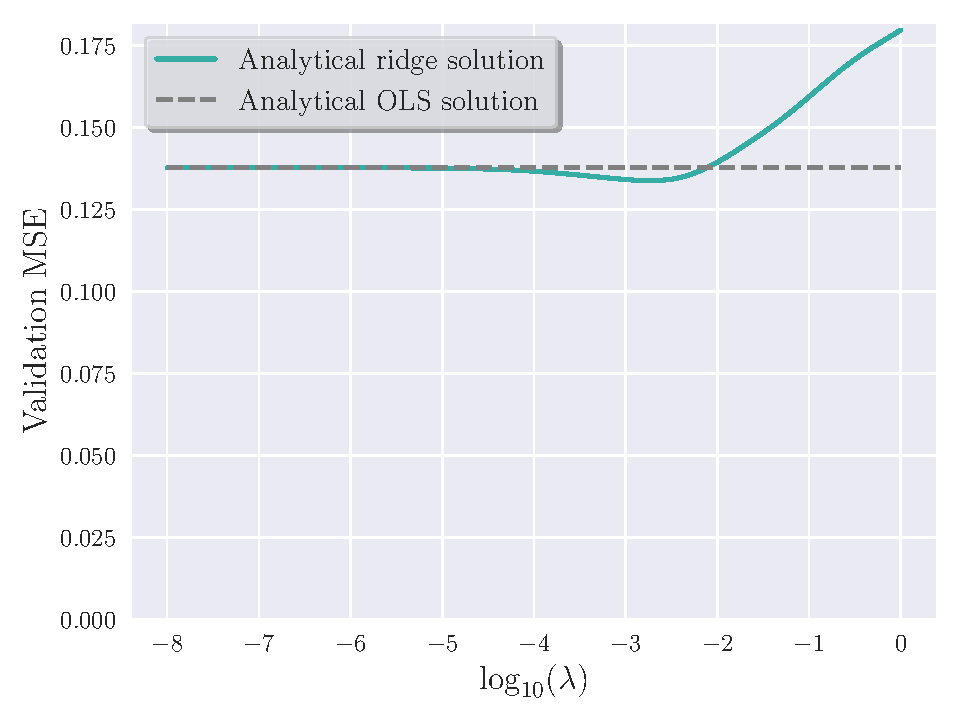
\includegraphics[width=\linewidth]{lmbda_plot_ana}
            \caption{Plot of the validation MSE found from optimising our linear regression parameters to the ridge cost function as a function of the penalisation parameter $\lambda$. The optimal MSE is 0.1338 with $\lambda = 0.002$.}
            \label[fig]{res:fig:ridge_ana}
        \end{figure}


\subsection{Neural Network and regression}
    \subsubsection{Varying Layers, Nodes, and Learning Rate}
        When varying the number of hidden layers (1,3,5), nodes in each layer (between 2-200), and learning rate (0.8-0.005), we found that the best MSE results, for each \# layers, came from the networks in table \cref{res:tab:heatmap_nodes}. 

        \renewcommand{\arraystretch}{1.25}
        \begin{table}[]
            \centering
            \begin{tabular}{r|c|c|c}
                \# Layers & Best network & $\eta$ &  MSE \\ \hline
                1         & \network{1}{50}            & 0.8    & 0.13              \\
                3         & \network{3}{200}            & 0.01   & 0.094             \\
                5         & \network{5}{200}            & 0.001  & 0.088             \\
                3, SciKit & \network{1}{10}            & 0.08   & 0.18              \\
            \end{tabular}
            \caption{Table of the best networks' MSE value.}
            \label[tab]{res:tab:heatmap_nodes}
        \end{table}
        \renewcommand{\arraystretch}{1}

        See \cref{res:fig:heatmap_nodes} for all results in heatmap. We see that increase in the \#layers leads to more networks that are unable to converge (see high MSE-values).  

        \begin{figure*}
            \begin{subfigure}{.49\textwidth}
                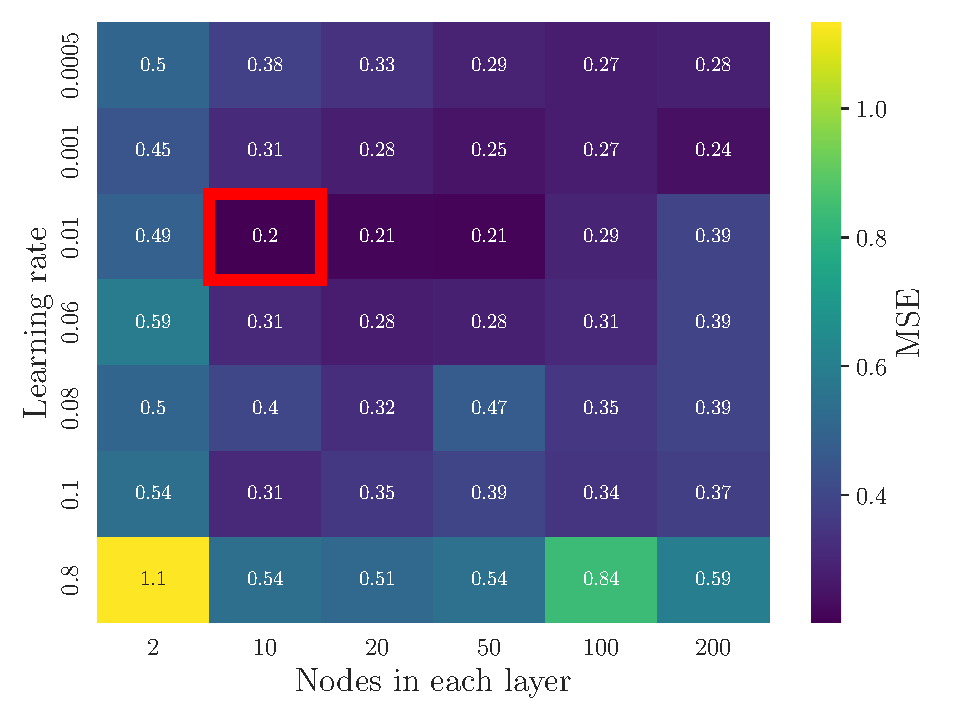
\includegraphics[width=\linewidth]{nodes_etas_heatmap_1.pdf}
                \caption{\textbf{1 Layer} The best result from \network{1}{50} MSE = 0.13.}
                \label[fig]{res:fig:1_lay}
            \end{subfigure}
            \hfill 
            \begin{subfigure}{.49\textwidth}
                \centering
                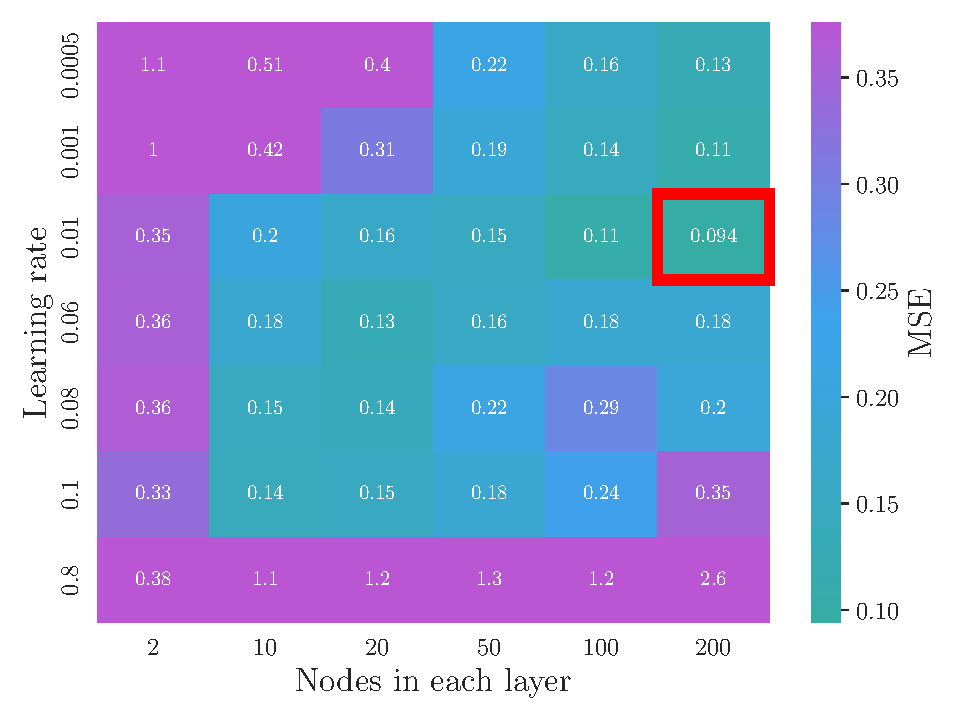
\includegraphics[width=\linewidth]{nodes_etas_heatmap_3.pdf}
                \caption{\textbf{3 Layers} The best result from \network{3}{200} MSE = 0.094.}
                \label[fig]{res:fig:3_lay}
            \end{subfigure}
            \hfill 
            \begin{subfigure}{.49\textwidth}
                \centering
                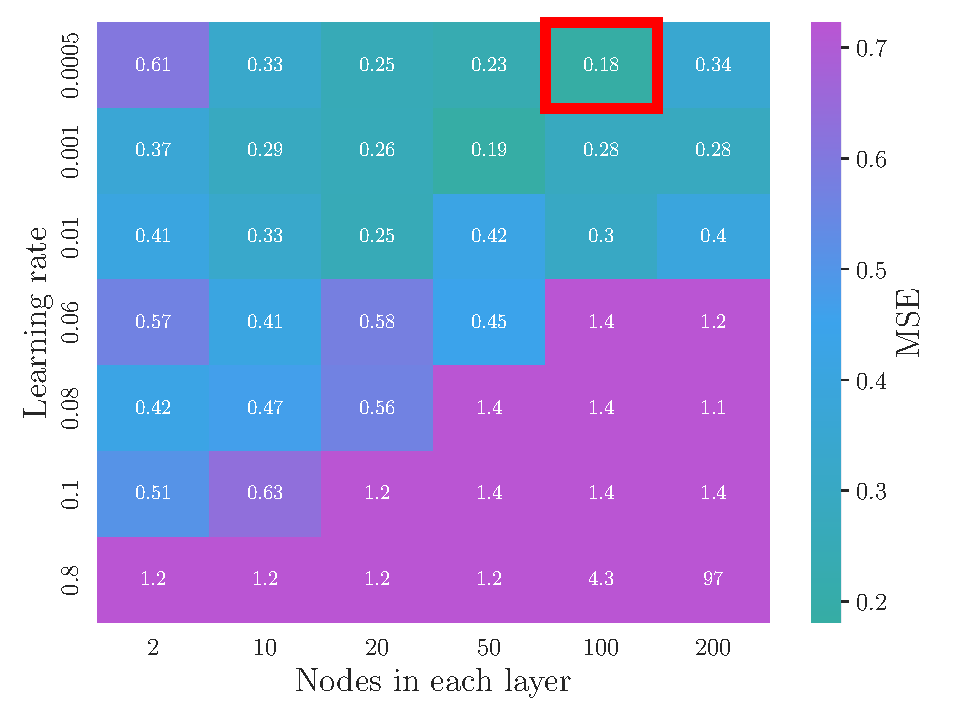
\includegraphics[width=\linewidth]{nodes_etas_heatmap_5.pdf}
                \caption{\textbf{5 Layers} The best result from \network{5}{200} MSE = 0.088.}
                \label[fig]{res:fig:5_lay}
            \end{subfigure}
            \hfill 
            \begin{subfigure}{.49\textwidth}
                \centering
                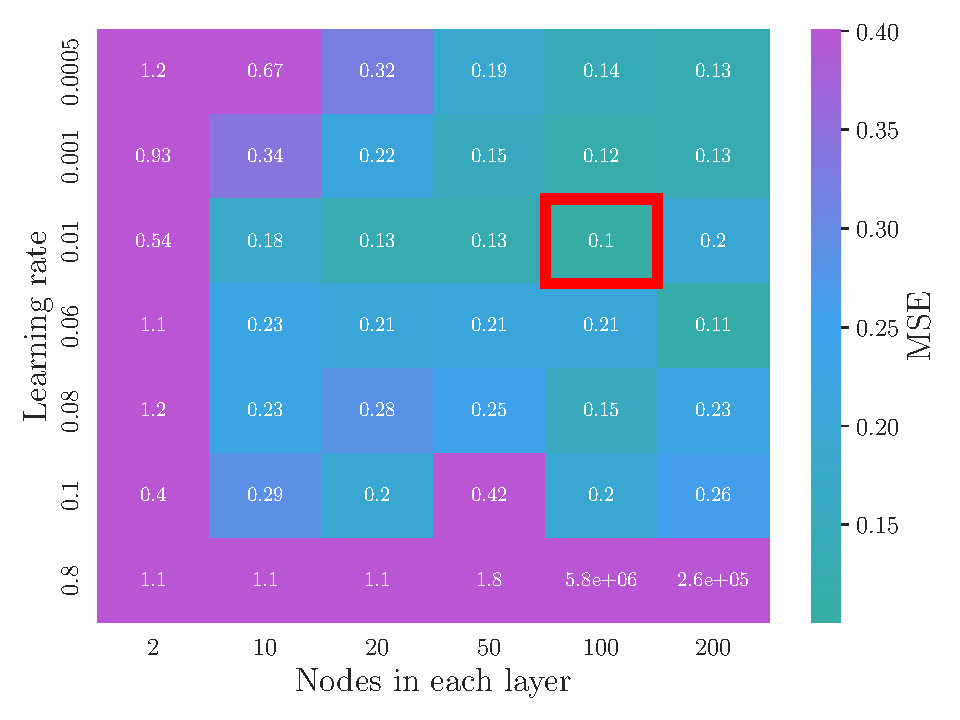
\includegraphics[width=\linewidth]{nodes_etas_heatmap_sk_3.pdf}
                \caption{\textbf{3 Layers SciKit-Learn} The best result from \network{3}{10} MSE = 0.18.}
                \label[fig]{res:fig:sk_3_lay}
            \end{subfigure}
            \caption{Heatmaps of the various networks constructed varying number nodes in each layer and learning rate for different number of layers. }
            \label[fig]{res:fig:heatmap_nodes}
        \end{figure*}


    \subsubsection{Exploring Activation Functions}
        The results in \cref{res:fig:plots_act_func} show that the implementation of activation functions affects the networks' performance. \cref{res:fig:act_funcs} illustrates that the shape of a network's predicted graph shares similarities with the graph of the implemented activation function; identity is linear, sigmoid and tanh are rather smooth, and ReLU and leaky ReLU are more discontinuous. The MSE values of the predictions are given in \cref{res:tab:act_funcs}. 

        \begin{table}[]
            \centering
            \begin{tabular}{r|l}
                \textbf{Activation Function} & \textbf{Validation MSE} \\ \hline
                identity                                                       & 0.113                                                    \\ 
                sigmoid                                                        & 0.013                                                    \\ 
                tanh                                                           & 0.014                                                    \\ 
                ReLU                                                           & 0.013                                                    \\ 
                leaky ReLU                                                     & 0.013                                                    \\ 
            \end{tabular}
            \caption{Table of the MSE values from the predictions in \cref{res:fig:act_funcs}.}
            \label[tab]{res:tab:act_funcs}
        \end{table}


        We notice that in the implementation of our network, the optimal network is still \network{5}{200} with the sidmoid activation function (from above). However, the \verb|scikit-learn| improves when changing from sigmoid to ReLU. There are now more non-converging networks and occurence of exploding gradients. 

        \begin{figure*}
            \begin{subfigure}{.49\textwidth}
                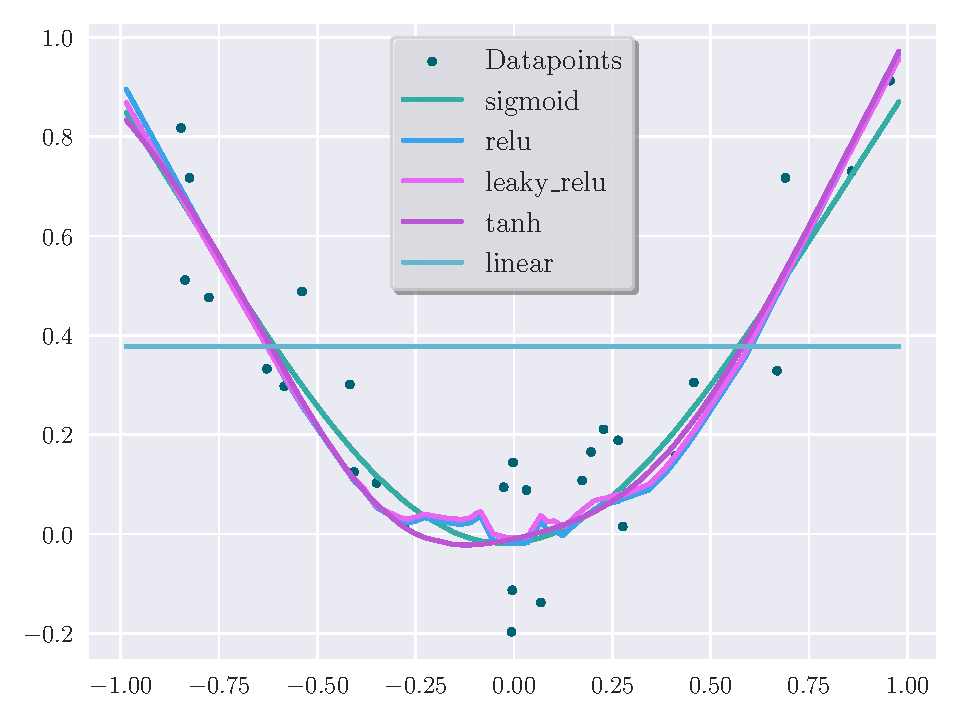
\includegraphics[width=\linewidth]{c_activations_2d_data.pdf}
                \caption{Networks with various activation functions trained $x^2 + \epsilon$ ($\epsilon \distas \normal{0}{0.1^2}$) with $x \in [-1,1]$ plotted.}
                \label[fig]{res:fig:act_funcs}
            \end{subfigure}
            \hfill 
            \begin{subfigure}{.49\textwidth}
                \centering
                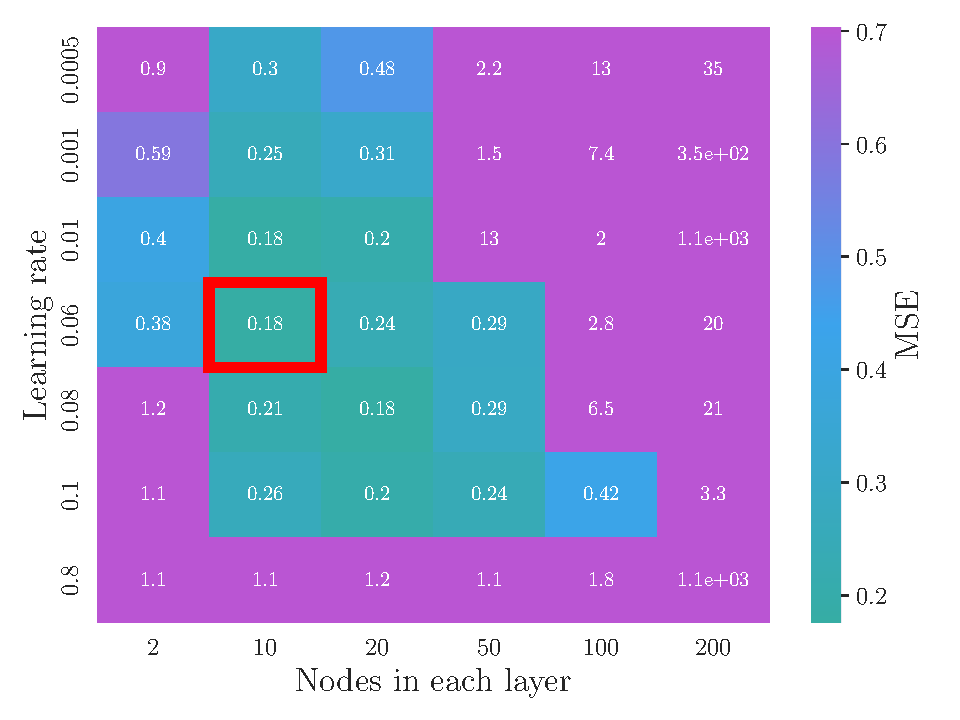
\includegraphics[width=\linewidth]{nodes_etas_heatmap_3_relu.pdf}
                \caption{ \textbf{3 layers, ReLU} activation function implemented. Best MSE value is 0.18.}
                \label[fig]{res:fig:relu}
            \end{subfigure}
            \hfill 
            \begin{subfigure}{.49\textwidth}
                \centering
                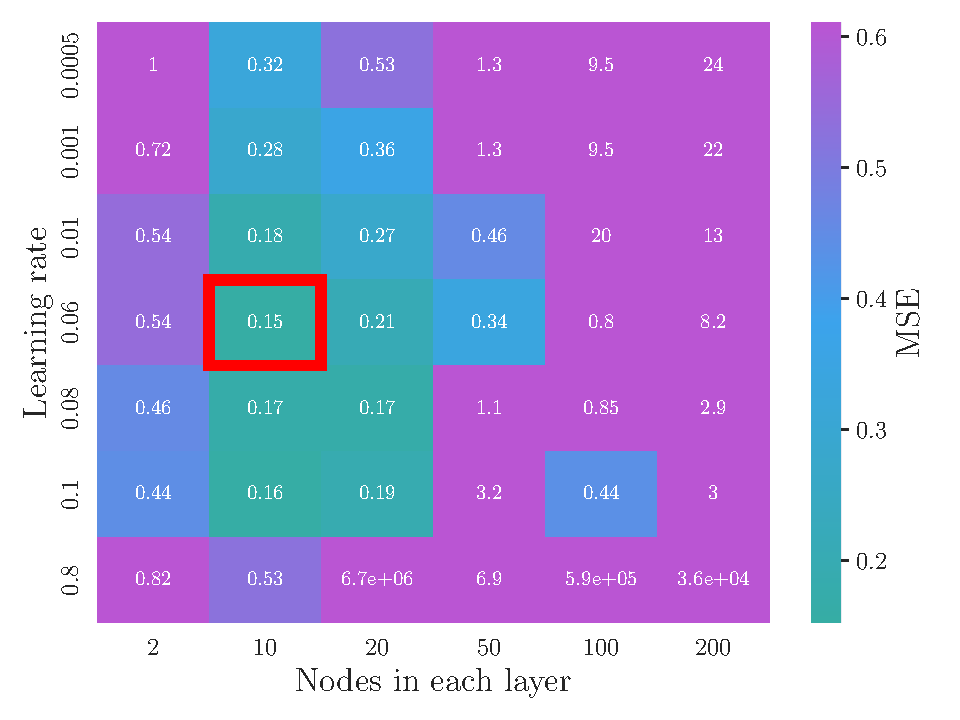
\includegraphics[width=\linewidth]{nodes_etas_heatmap_3_lrelu.pdf}
                \caption{ \textbf{3 layers, Leaky ReLU} activation function implemented. Best MSE value is 0.15.}
                \label[fig]{res:fig:l_relu}
            \end{subfigure}
            \hfill 
            \begin{subfigure}{.49\textwidth}
                \centering
                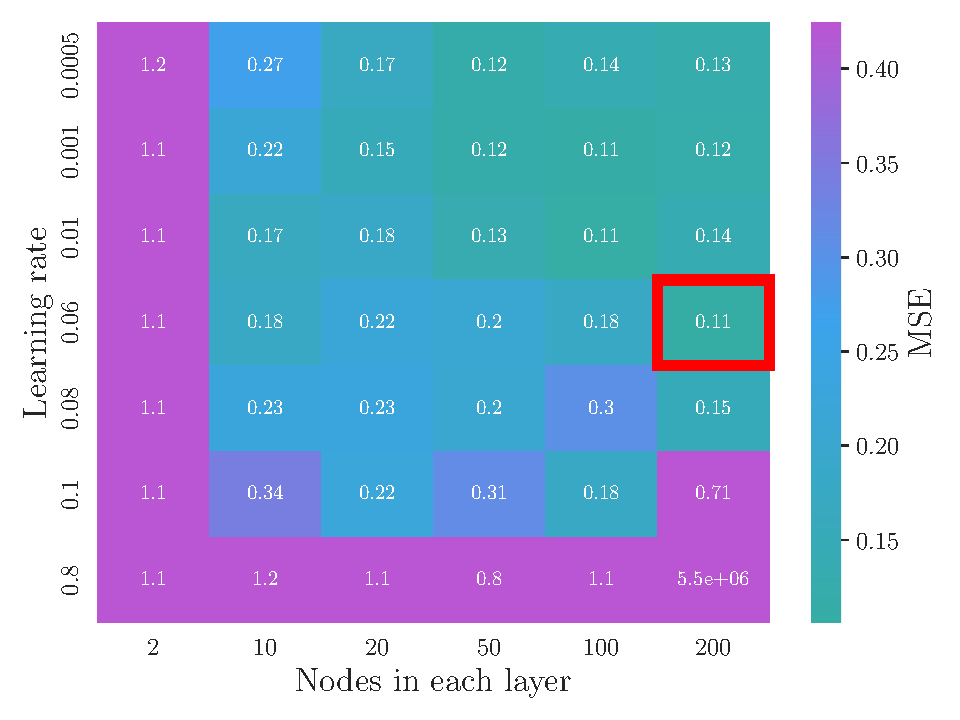
\includegraphics[width=\linewidth]{nodes_etas_heatmap_sk_3_relu.pdf}
                \caption{ \textbf{3 layers, SciKit-Learn with ReLU} activation function implemented. Best MSE value is 0.11.}
                \label[fig]{res:fig:sk_relu}
            \end{subfigure}
            \caption{Plots from exploration of the activation functions.}
            \label[fig]{res:fig:plots_act_func}
        \end{figure*}

    \subsubsection{Exploring Regularisation}
        From \cref{res:fig:regularisation_2D} the $\lambda$ yielding the lowest MSE value was $\lambda = 10^{-4.1}$ giving  an MSE of 0.078. This was for the network with $\eta = 0.001$. When also varying the learning rate (see \cref{res:fig:regularisation_heatmap}), the optimal network also had $\eta = 0.001$ and now $\lambda = 10^{-4}$. 
        \begin{figure*}            
            \begin{subfigure}{.49\textwidth}
                \centering
                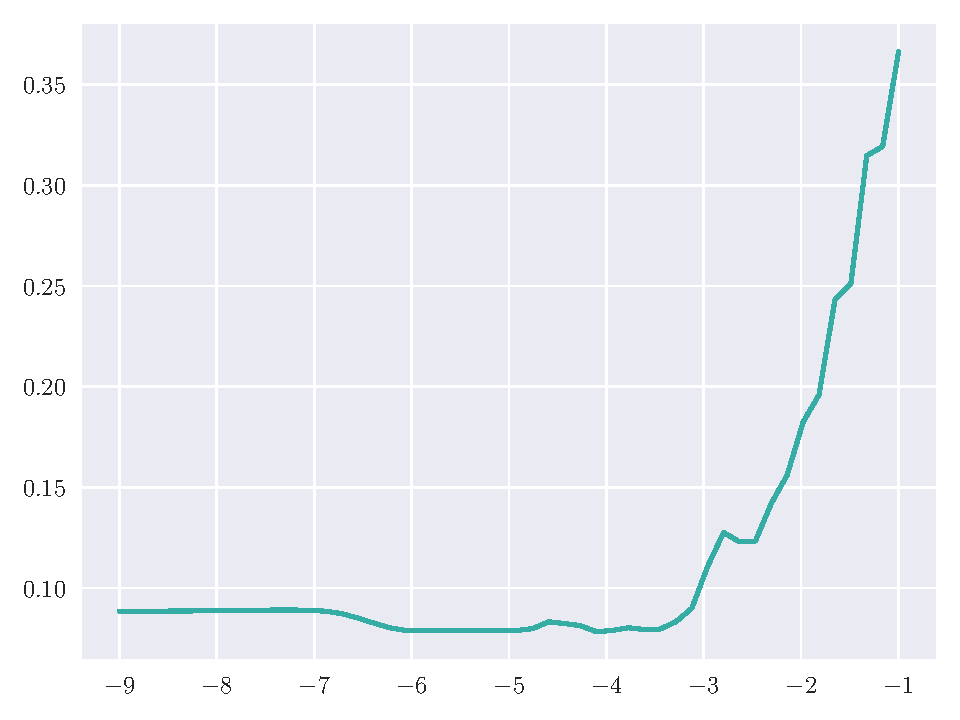
\includegraphics[width=\linewidth]{lmbdas_NN_reg.pdf}
                \caption{ Plot of the validation MSE as a function of the regularisation, $\lambda$s. \network{5}{200}, with sigmoid and $\eta = 0.001$.}
                \label[fig]{res:fig:regularisation_2D}
            \end{subfigure}
            \begin{subfigure}{.49\textwidth}
                \centering
                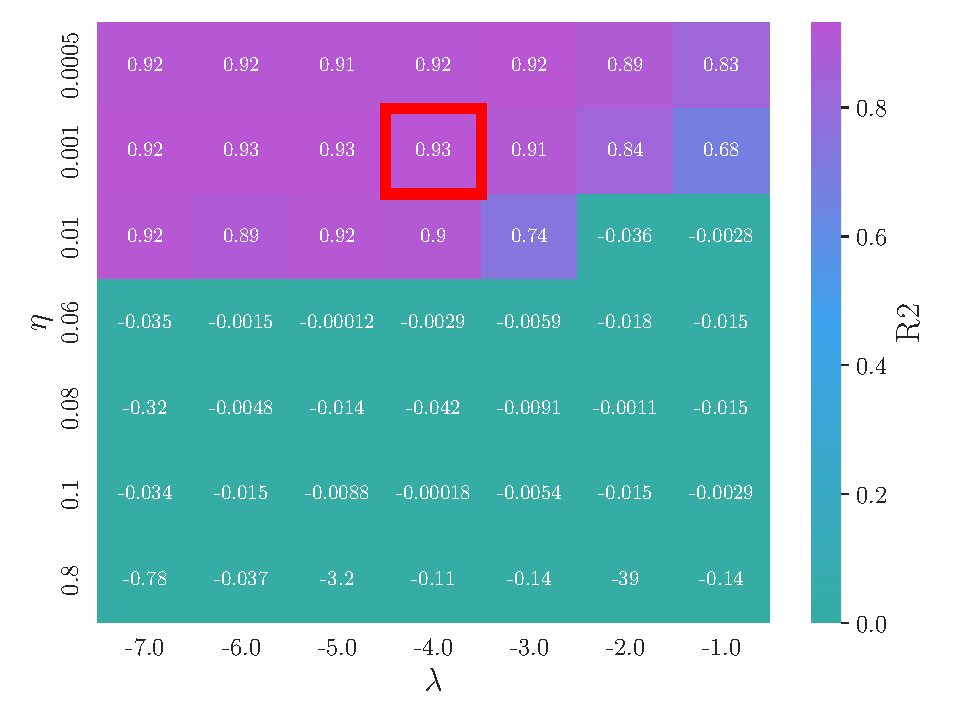
\includegraphics[width=\linewidth]{lmbdas_etas_heatmap_5_2.pdf}
                \caption{Heatmap of various $\eta$s, $\lambda$s and the produced R2 score. \network{5}{200}, with sigmoid and $\eta = 0.001$.}
                \label[fig]{res:fig:regularisation_heatmap}
            \end{subfigure}
            \caption{Results from exploring an added regularisation hyperparameter.}
            \label[fig]{res:fig:regularisation}
        \end{figure*}
        

    \subsubsection{Terrain data}
        In \cref{res:fig:terrain} the plots of the true and predicted Nicaraguan terrains are presented. The MSE of the network-predicted was 0.078 and of the OLS model 0.171. We saw, qualitatively and quantitatively, that the network outperformed the linear regression. By eye, it seemed also that the network replicated many of the key elements of the true terrain data.
        \begin{figure}
            \begin{subfigure}{.49\textwidth}
                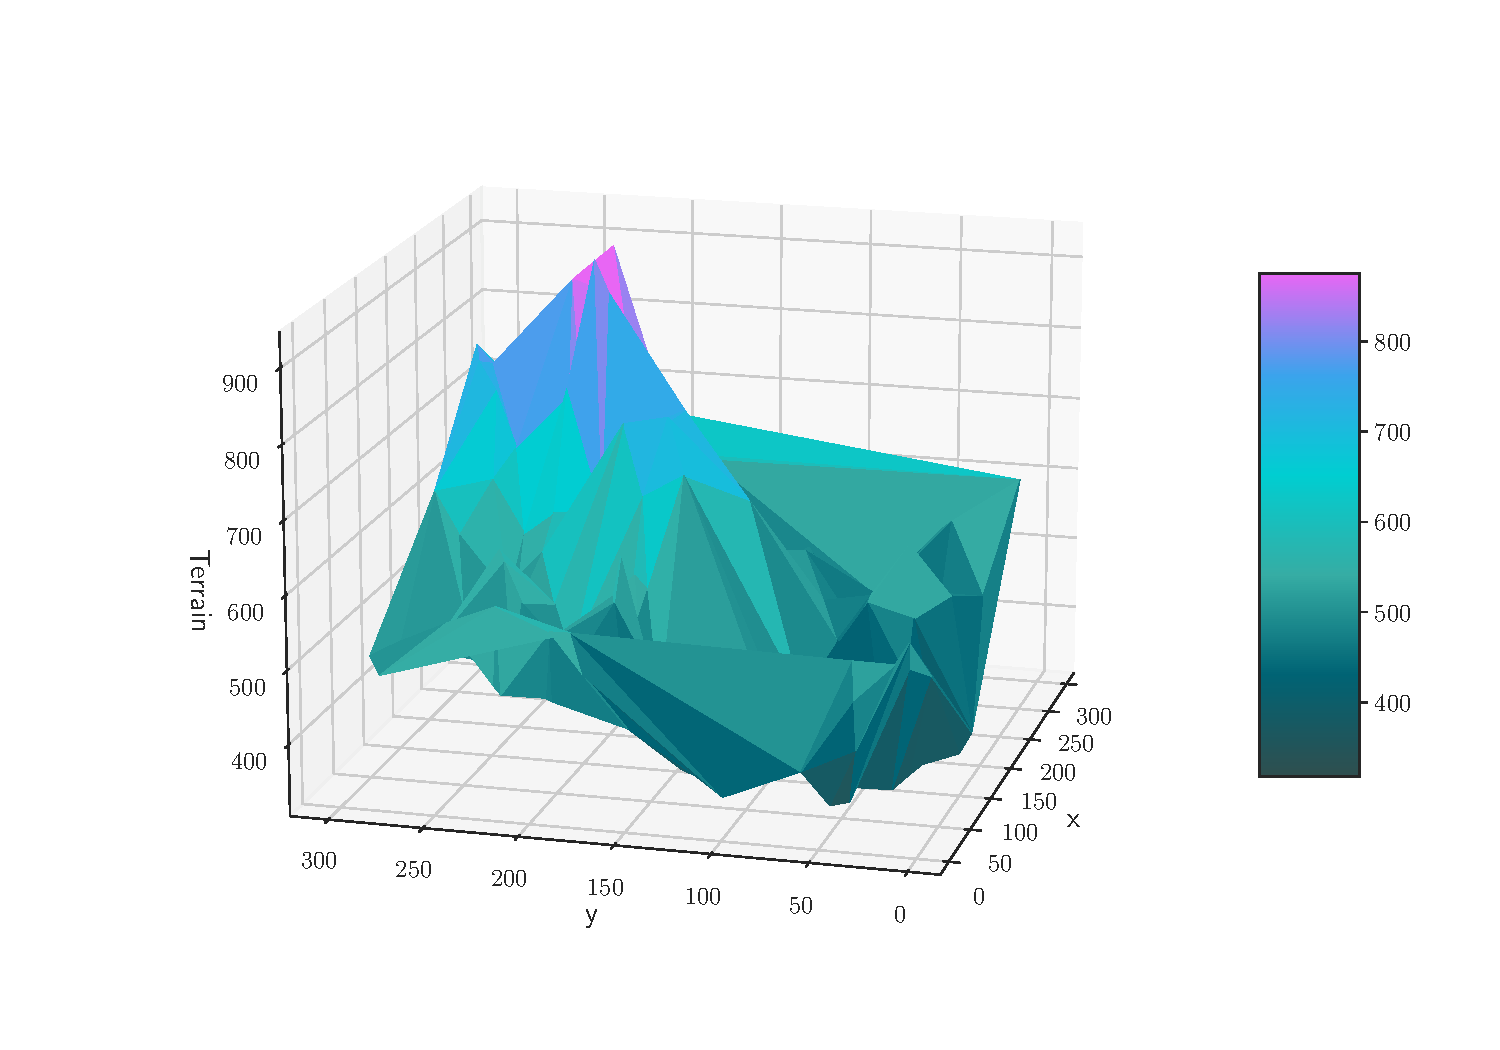
\includegraphics[width=\linewidth]{terrain_test.pdf}
                \caption{\textbf{True data} from the Nicaraguan terrain.}
                \label[fig]{res:fig:terrain_test}
            \end{subfigure}
            \hfill 
            \begin{subfigure}{.49\textwidth}
                \centering
                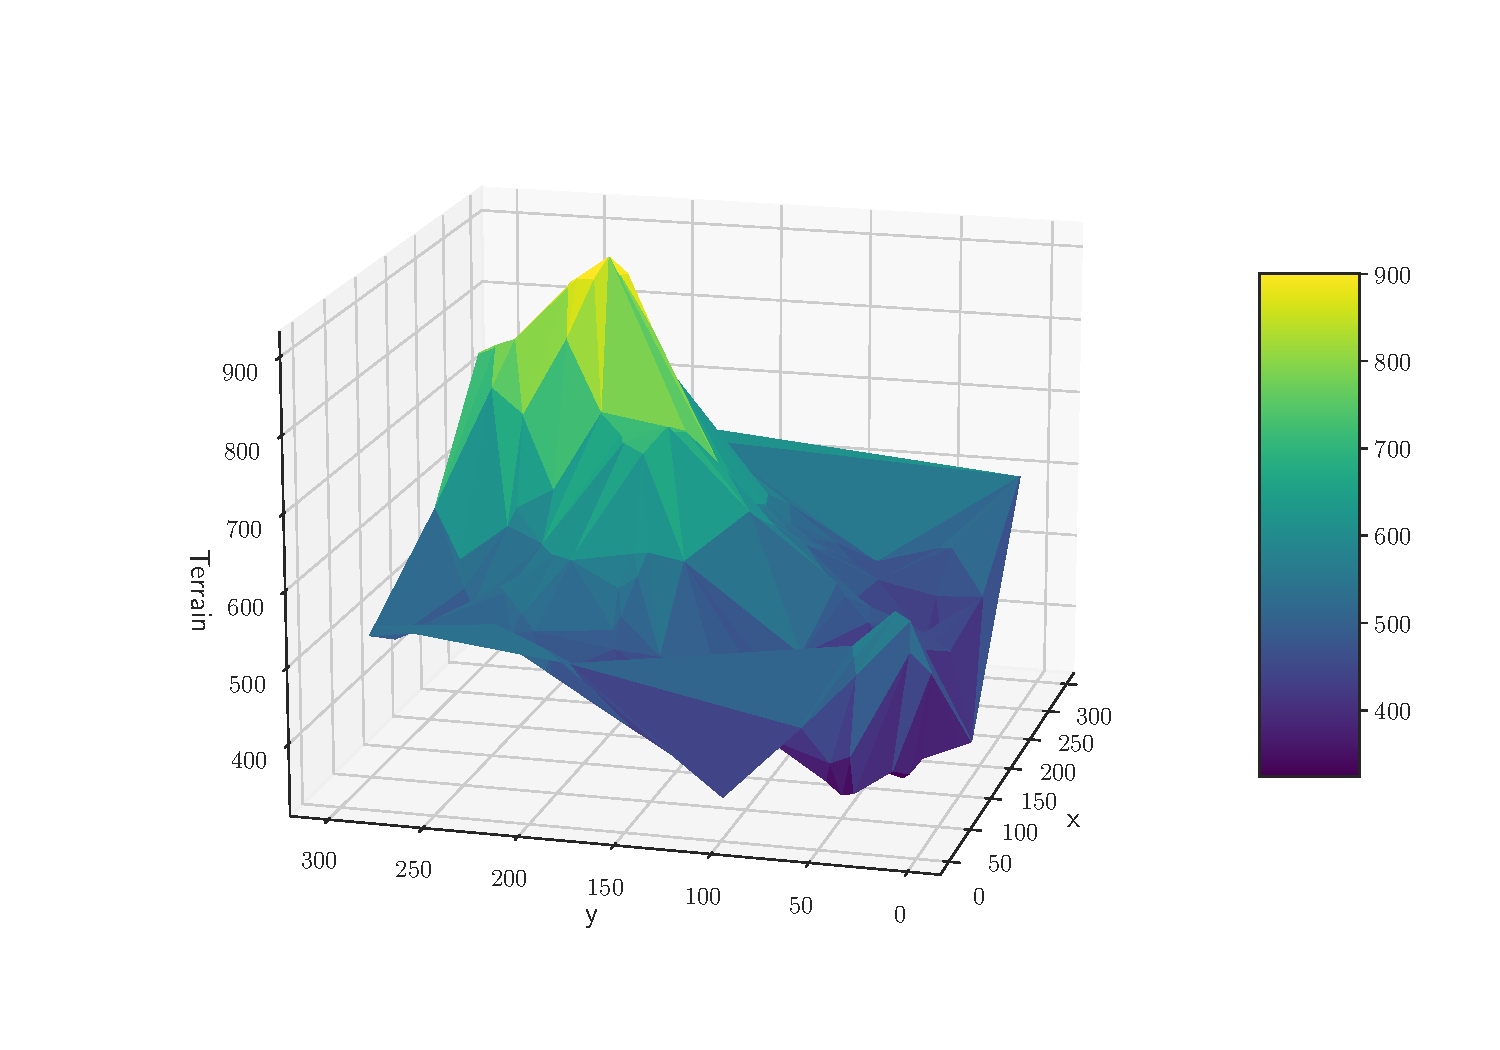
\includegraphics[width=\linewidth]{terrain_predicted.pdf}
                \caption{\textbf{Network-predicted} Nicaraguan terrain. MSE = 0.078}
                \label[fig]{res:fig:terrain_pred_NN}
            \end{subfigure}
            \hfill 
            \begin{subfigure}{.49\textwidth}
                \centering
                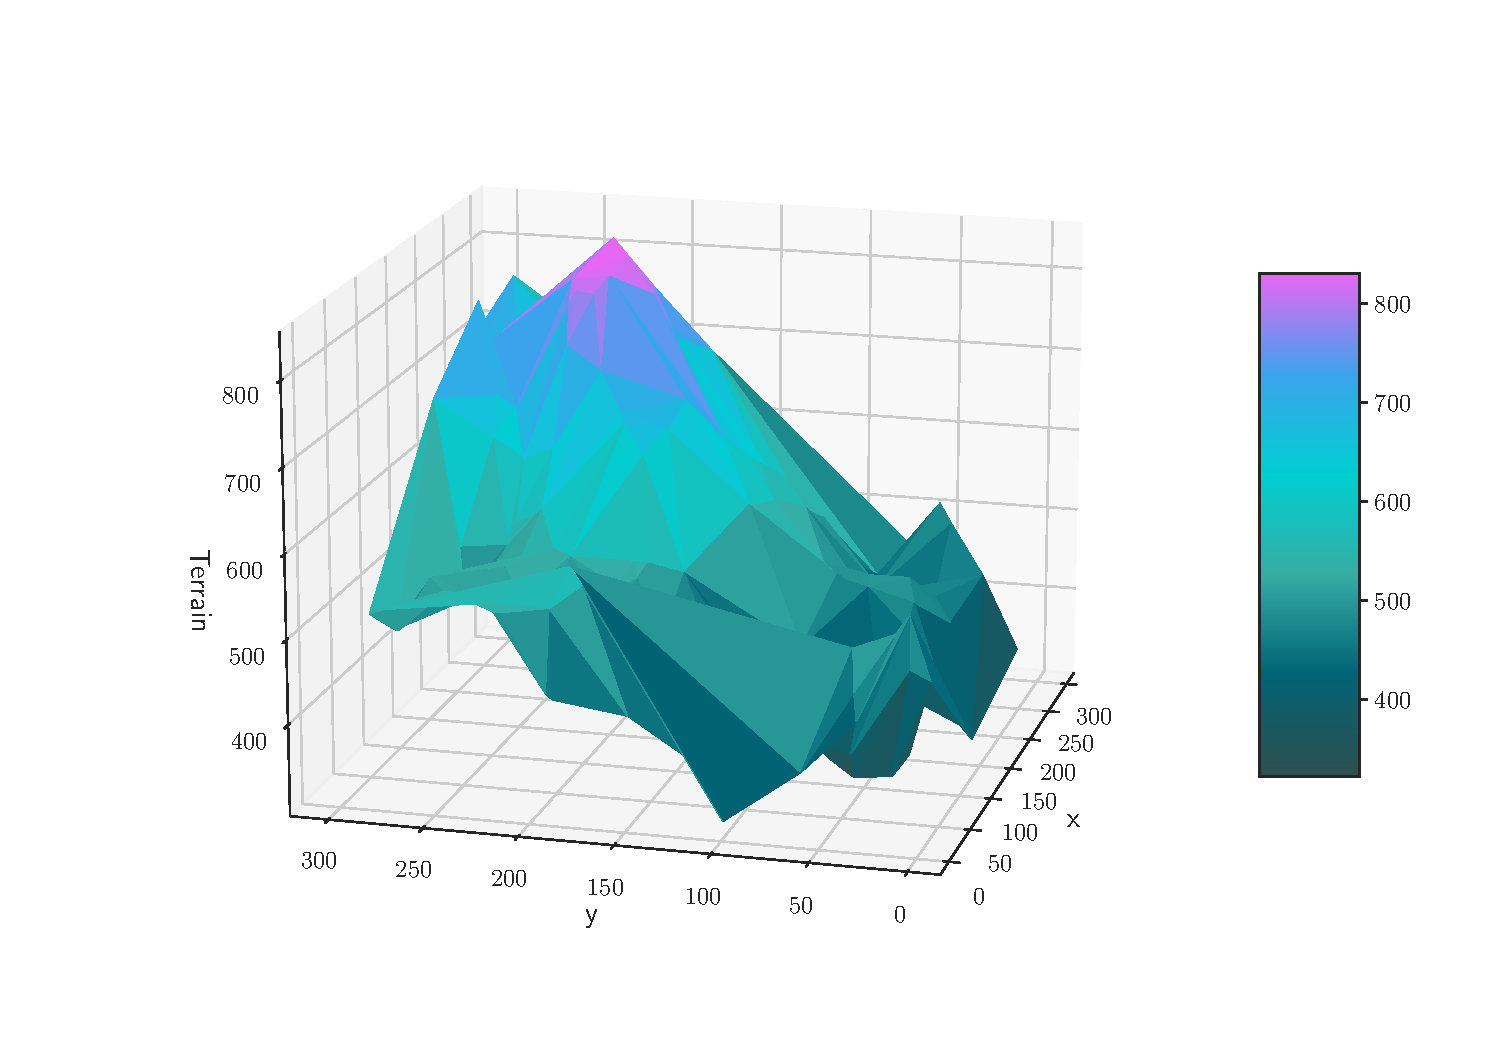
\includegraphics[width=\linewidth]{terrain_OLS.pdf}
                \caption{\textbf{OLS-predicted} Nicaraguan terrain. $p=11$. MSE= 0.171}
                \label[fig]{res:fig:terrain_pred_OLS}
            \end{subfigure}
            \caption{Plots of the true and predicted Nicaraguan terrains.}
            \label[fig]{res:fig:terrain}
        \end{figure}
        


\subsection{Wisconsin Breast Cancer}
    \subsubsection{Logistic regression}
        The different optimisation algorithms from our library of gradient decent methods were applied to optimise the BCE cost function without penalisation \cref{the:eq:logreg_cost_function} using Logistic regression. This is presented in \cref{res:fig:logreg_GD_opt} for GD methods with and without momentum, while SGD based methods are presented in \cref{res:fig:logreg_SGD_opt}. We found that every method, given the correct learning rate and number of iterations, managed to obtain an accuracy above $0.9$.  
        
        Plain gradient decent running 5 iterations performed the worst, at best acheiving an accuracy of $0.958$ at $\eta = 0.859$. However, when allowed to run for 50 iterations, accuracy scores $> 0.95$ were achieved across all learning rates. The addition of momentum made the optimisation converge faster, where the case for 50 iterations is especially stable. In the domain of SGD based methods, both Adam and AdaGrad SGD out-competed plain SGD for 5 epochs. However, when allowed to run for 50 epochs, plain SGD also managed to converge acheiving accuracy scores $> 0.95$ across all learning rates.
        
        Validation accuracies calculated while optimising using GD and SGD based methods are presented in \cref{res:fig:logreg_under_optimazation}. Adam SGD and mGD achieved an accuracy of $~0.95$ using just a few iterations, while again GD and SGD performed the worst.  

        \begin{figure}
            \begin{subfigure}{.49\textwidth}
                \centering
                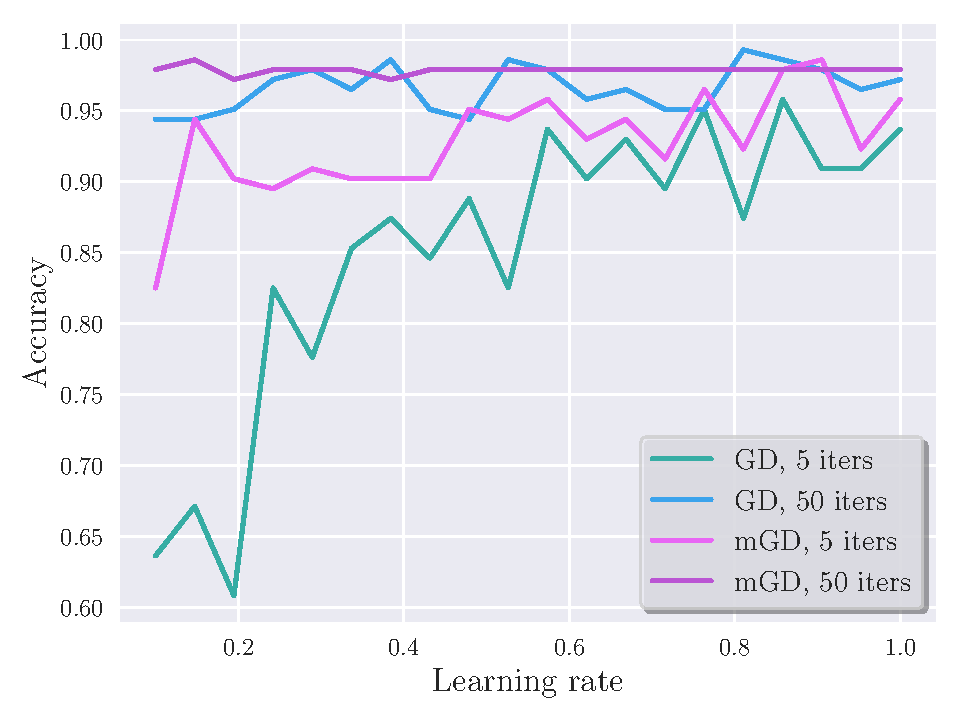
\includegraphics[width=\linewidth]{logreg_GD.pdf}
                \caption{Showing accuracy as a function of learning rate, optimised using GD with ($\gamma = 0.8$) and without momentum for 5 and 50 iterations.}
                \label[fig]{res:fig:logreg_GD_opt}
            \end{subfigure}
            \begin{subfigure}{.49\textwidth}
                \centering
                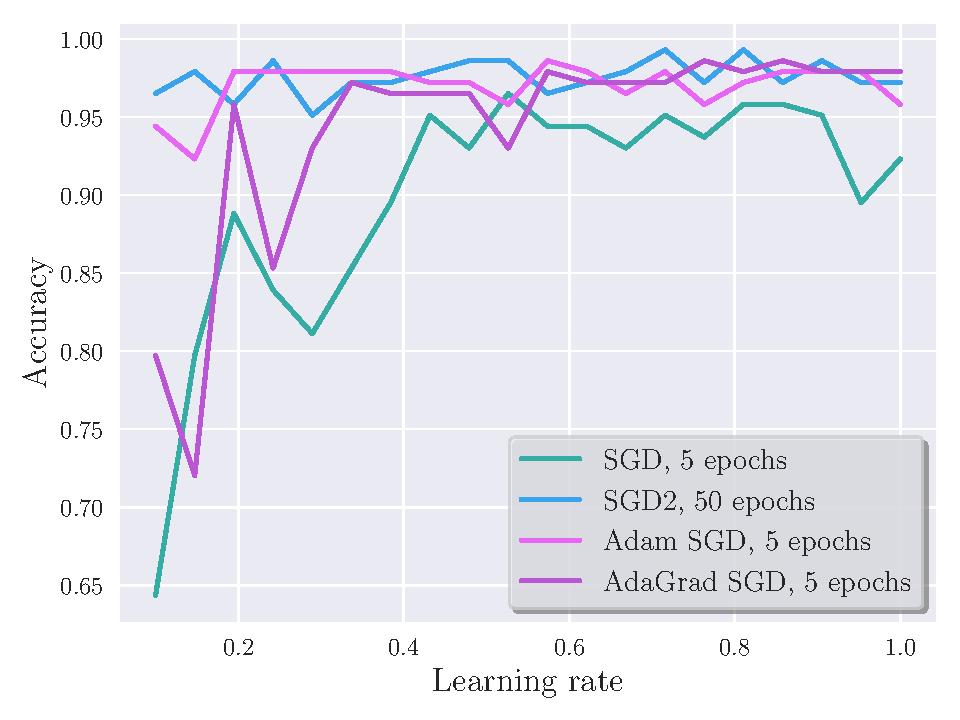
\includegraphics[width=\linewidth]{logreg_SGD.pdf}
                \caption{Showing accuracy as a function of learning rate, optimised plain, Adam ($\beta_1 = 0.9, \beta_2 = 0.99$) and AdaGrad SGD while varying the number of epochs. For all optimisations, a batch size of 200 was used.}
                \label[fig]{res:fig:logreg_SGD_opt}
            \end{subfigure}
            \begin{subfigure}{.49\textwidth}
                \centering
                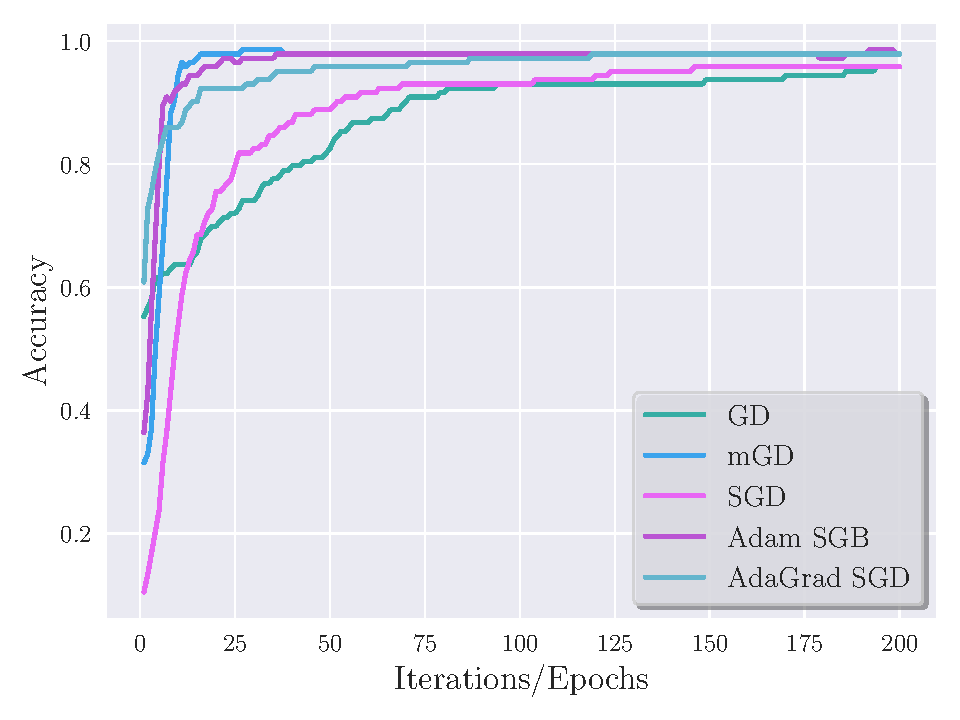
\includegraphics[width=\linewidth]{logreg_acc_during_optimazation.pdf}
                \caption{Showing accuracy as a function of iterations/epochs. All methods used $\eta = 0.05$, with Adam having $\beta_1 = 0.9, \beta_2 = 0.99$ and momentum GD $\gamma = 0.8$.}
                \label[fig]{res:fig:logreg_under_optimazation}
            \end{subfigure}
        \end{figure}

        Using Adam SGD with $\beta_1 = 0.9, \beta_2 = 0.99$ as an optimisation algorithm, the validation accuracy varied for both penalisation $\lambda$ and learning rate $\eta$ is shown in \cref{res:fig:logreg_penalisation}. We found that multiple models gave the same optimal validation accuracy, for both low penalisation $(\lambda = 10^{-6})$ and higher penalisation $(\lambda = 10^{-1.5})$. The $(\lambda = 10^{-6})$ used a learning rate of $\eta = 0.13$ while the $\lambda = 10^{-1.5}$ models used higher learning rates in the range $\eta \in [0.25, 0.5]$. When using the logistic regression implementation from \verb|scikit-learn|, we found a validation accuracy score of 0.986 without any penalisation, which lay in the vicinity of the results obtained from our own implementation.
 

        \begin{figure}
            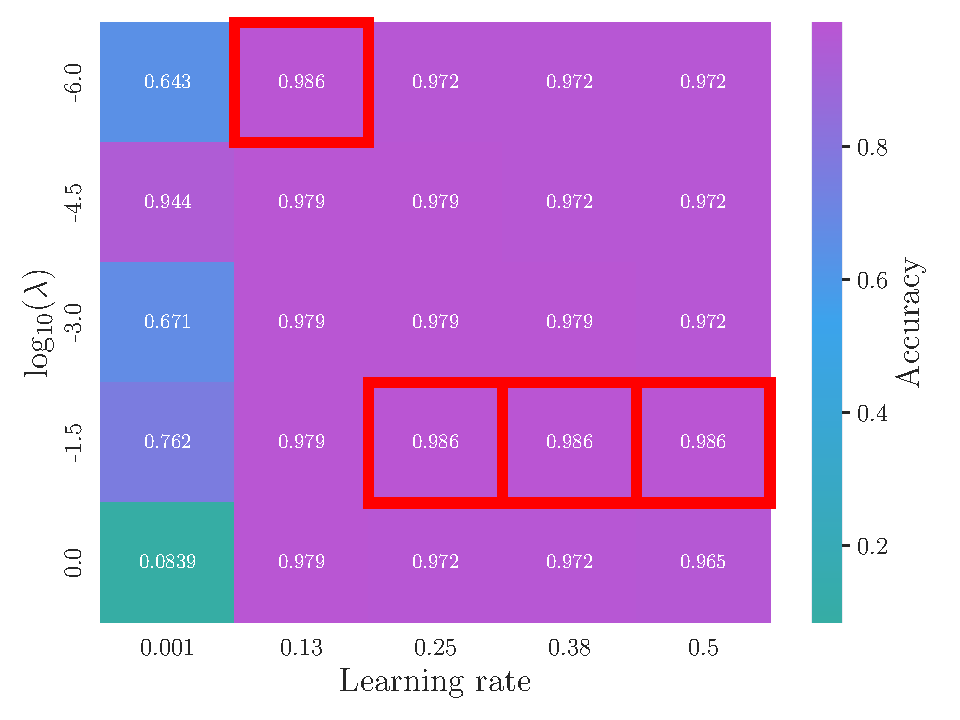
\includegraphics[width=\linewidth]{logreg_penalisation.pdf}
            \caption{Validation accuracy for logistic regression as a function of learning rate and penalisation parameter $\lambda$. Largest accuracy of $A = 0.986$ found at $\lambda = 10^{-6}$ using $\eta = 0.13$ and $\lambda = 10^{-1.5}$ with $\eta = 0.25, 0.38$ and $0.50$}
            \label[fig]{res:fig:logreg_penalisation}
        \end{figure}

    \subsubsection{Classification Neural Network}
        The validation accuracy of the network models \network{1}{5}, \network{1}{10}, \network{2}{5} and \network{3}{5} using different hidden activation functions is shown in \cref{res:fig:clf_afs}, with the optimal accuracy scores presented in \cref{res:tab:accuracy_score_activation_functions}. For \network{1}{5} \cref{res:fig:clf_af_N_1_5}, the sigmoid function seemed always to perform the best, with only Leaky ReLU matching its best accuracy of 0.993 for $\eta = 0.23$. From \cref{res:fig:clf_af_N_1_10}, \network{1}{10} also performed the best using the sigmoid function, with hyperbolic tangent being the second best. For this structure, both ReLU and Leaky ReLU performed worse across all learning rates tested here. The two and three layer structures \network{2}{5} and \network{3}{5} seen in \cref{res:fig:clf_af_N_2_5} and \cref{res:fig:clf_af_N_3_5} respectively was less clear on the preferred hidden activation function. \network{2}{5} seemed to be more learning rate dependent when choosing a hidden activation function, where all four functions tried here yielded an accuracy of $0.993$ for different learning rates. Increasing the complexity to \network{3}{5} did not yield any increase in validation accuracy, but the results from the sigmoid function was particularly stable in this case.  

        Due to the stable performance of the \network{1}{5} structure, we chose to include this in the penalisation optimisation. To include slightly deeper structure, \network{2}{5} was also chosen, since there were no significant increase in validation accuracy when moving to \network{3}{5}. Using the sigmoid and hyperbolic tangent hidden activation functions, the $\lambda$ and $\eta$ optimisation for these two structures is shown in \cref{res:fig:clf_heatmaps}. The \network{1}{5} structure had its best validation accuracy when using the sigmoid function for learning rates $\eta = 0.08, 0.1$ with penalisations $\lambda = 10^{-3.5}, 10^{-5.75}$ and $10^{-8.0}$ as seen in \cref{res:fig:clf_heatmap_N_1_5_sig}. The slightly lower accuracy of $0.986$ was found using hyperbolic tangent function as seen in \cref{res:fig:clf_heatmap_N_1_5_tanh}, with optimal parameters $\lambda =10^{-5.75},  10^{-8.0}$ for $\eta = 0.05$ and $\lambda = 10^{-3.5}$ for $\eta = 0.08$. When moving to the structure \network{2}{5}, both the sigmoid and hyperbolic tangent functions yielded an accuracy of $0.993$ as seen in \cref{res:fig:clf_heatmap_N_2_5_sig} and \cref{res:fig:clf_heatmap_N_2_5_tanh} respectively. For the sigmoid, five sets of hyperparameters gave this accuracy: $\lambda = 10^{-8.0}, 10^{-5.75}$ for $\eta = 0.03, 0.05$ in addition to $\lambda = 10^{-5.75}$ for $\eta = 0.1$. The hyperbolic tangent only had a single set, $\lambda = 10^{-3.5}$ for $\eta = 0.03$.
        Lastly, using \verb|scikit-learn|'s neural network implementation, the \network{2}{5} structure using sigmoid activation function for both the hidden and output layer yielded a validation accuracy of 0.986 for multiple penalisation and learning rates, as shown in \cref{res:fig:clf_heatmap_sklearn}. Again, the obtained validation accuracy scores are in the vicinity of the results from our own +implementation.

        \begin{table}
            \begin{tabular}{l|l|l|l|l}
                \network{1}{5} & \network{1}{10} & \network{2}{5} & \network{3}{5} & $f_H$       \\
                \hline
                0.993             & 0.993              & 0.993             & 0.986             & sigmoid    \\
                0.986             & 0.986              & 0.993             & 0.993             & Tanh       \\
                0.986             & 0.979              & 0.993             & 0.986             & ReLU       \\
                0.993             & 0.979              & 0.993             & 0.986             & Leaky ReLU
            \end{tabular}
            \caption{The optimal validation accuracy scores calculated using different network structures and hidden activation functions $f_H$, across different learning rates. Multiple learning rates correspond to the same accuracy score.}
            \label[tab]{res:tab:accuracy_score_activation_functions}        
        \end{table}

        \begin{figure*}
            \begin{subfigure}{.49\textwidth}
                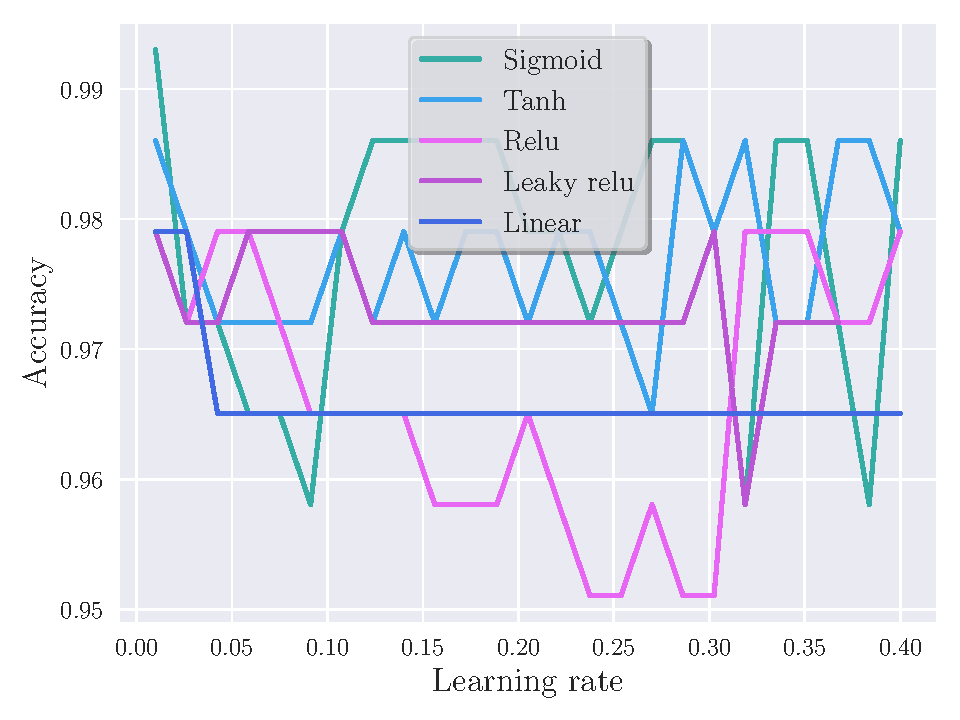
\includegraphics[width=\linewidth]{clasf_activation_functions1.pdf}
                \caption{Network \network{1}{5}, plotted for $\eta \in [ 0.1, 0.4 ]$ using 8 linearly spaced points}
                \label[fig]{res:fig:clf_af_N_1_5}
            \end{subfigure}
            \hfill 
            \begin{subfigure}{.49\textwidth}
                \centering
                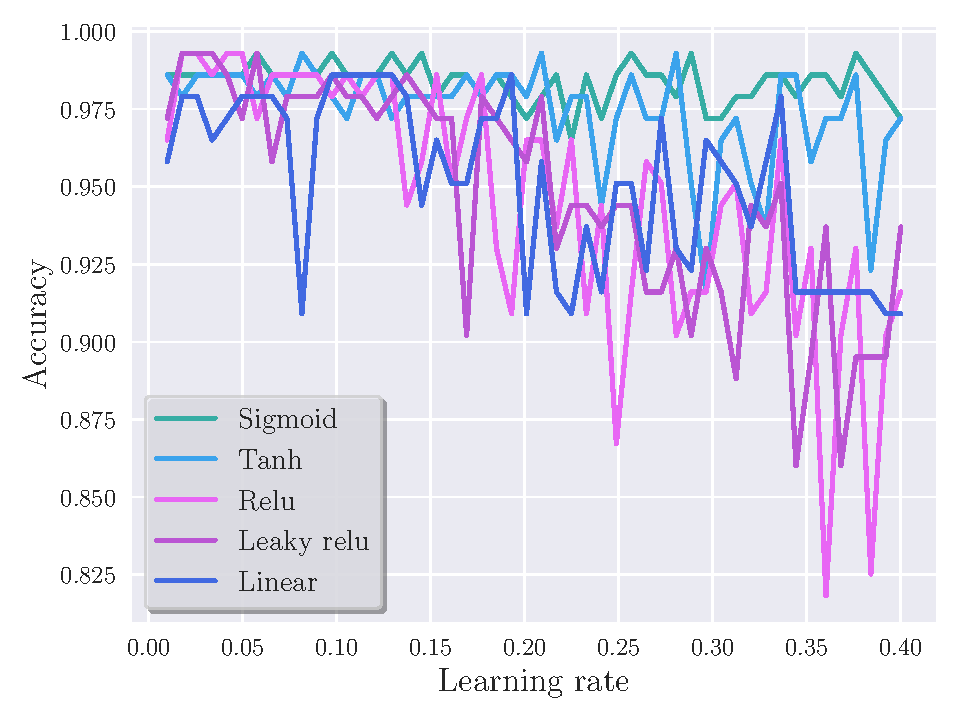
\includegraphics[width=\linewidth]{clasf_activation_functions2.pdf}
                \caption{Network \network{1}{10}, plotted for $\eta \in [ 0.01, 0.01 ]$ using 8 linearly spaced points}
                \label[fig]{res:fig:clf_af_N_1_10}
            \end{subfigure}
            \hfill 
            \begin{subfigure}{.49\textwidth}
                \centering
                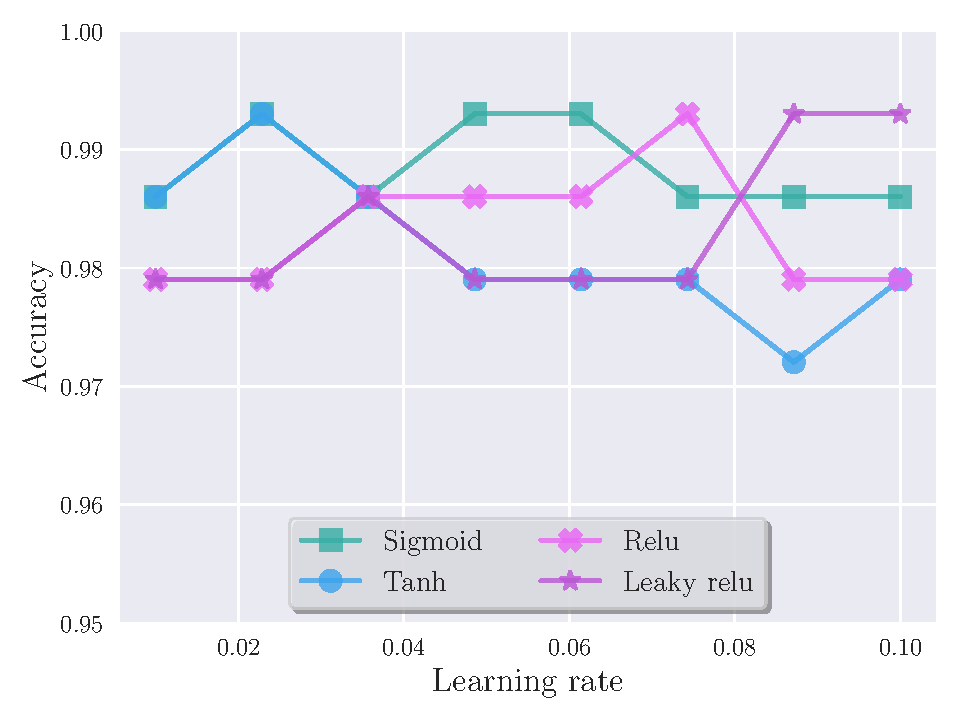
\includegraphics[width=\linewidth]{clasf_activation_functions3.pdf}
                \caption{Network \network{2}{5}, plotted for $\eta \in [ 0.01, 0.01 ]$ using 8 linearly spaced points}
                \label[fig]{res:fig:clf_af_N_2_5}
            \end{subfigure}
            \hfill 
            \begin{subfigure}{.49\textwidth}
                \centering
                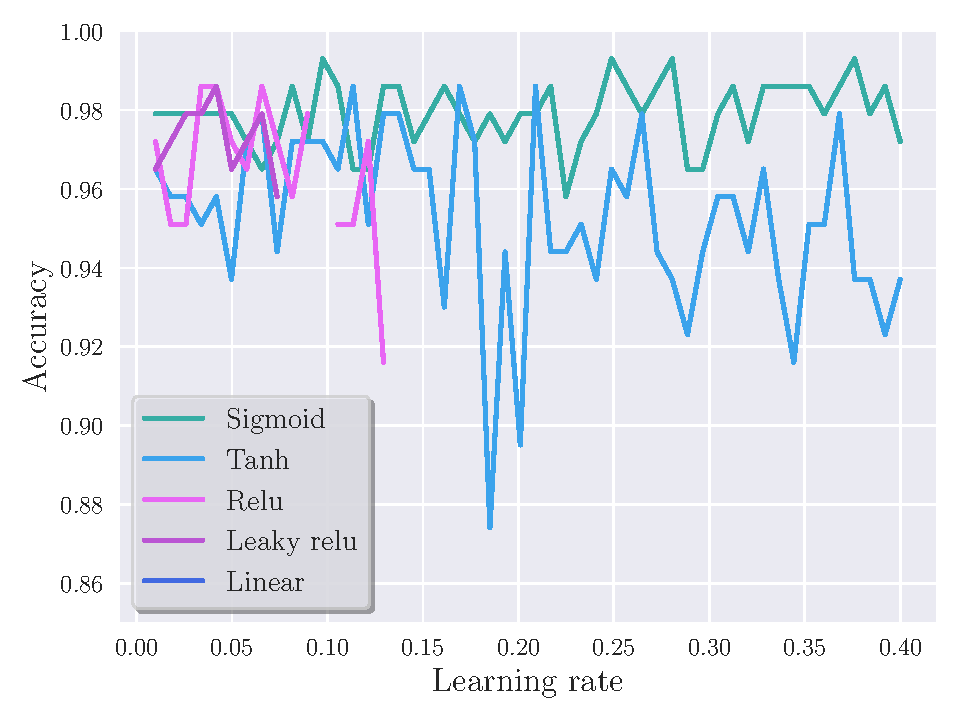
\includegraphics[width=\linewidth]{clasf_activation_functions4.pdf}
                \caption{Network \network{3}{5}, plotted for $\eta \in [ 0.01, 0.01 ]$ using 8 linearly spaced points}
                \label[fig]{res:fig:clf_af_N_3_5}
            \end{subfigure}
            \caption{Plots of the accuracy score against learning rate for different activation functions for used for the hidden layer(s). Different network models have been used for the four plots. The AdaGrad algorithm with momentum $\gamma = 0.8$ has been used for optimisation, running 100 epochs with a batch size of 200.}
            \label[fig]{res:fig:clf_afs}
        \end{figure*}

        \begin{figure*}
            \begin{subfigure}{.49\textwidth}
                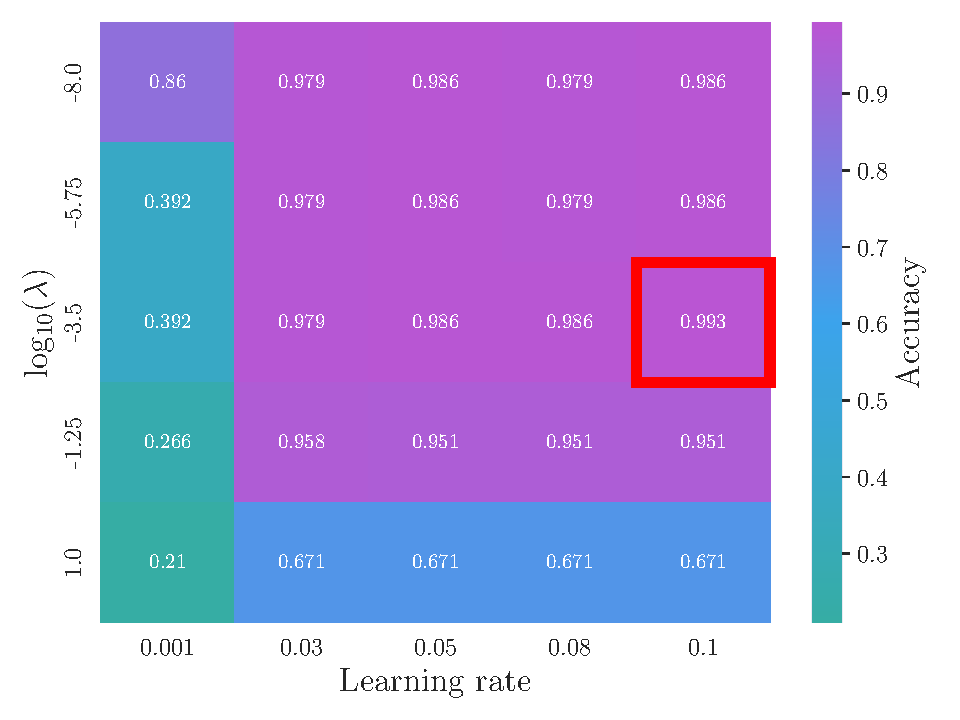
\includegraphics[width=\linewidth]{lmbda_lr_struct0_sigmoid.pdf}
                \caption{Network \network{1}{5} with a sigmoid activation function for the hidden layer. Multiple maxima was found with an accuracy of $0.993$}
                \label[fig]{res:fig:clf_heatmap_N_1_5_sig}
            \end{subfigure}
            \hfill
            \begin{subfigure}{.49\textwidth}
                \centering
                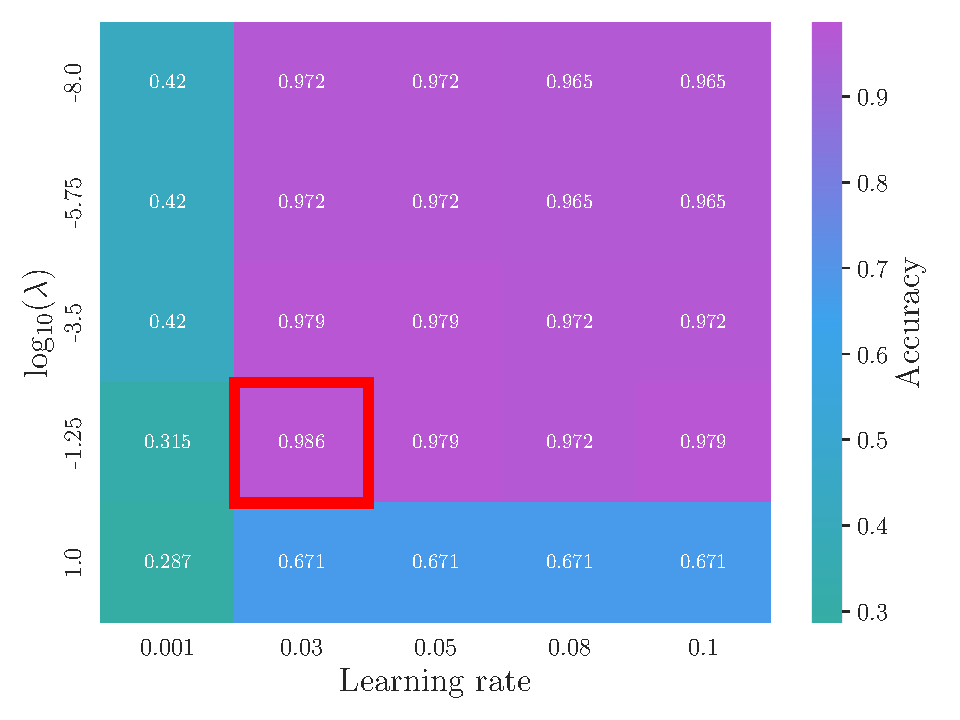
\includegraphics[width=\linewidth]{lmbda_lr_struct0_tanh.pdf}
                \caption{Network \network{1}{5} with a hyperbolic tangent activation function for the hidden layer. Multiple maxima was found with an accuracy of $0.986$.}
                \label[fig]{res:fig:clf_heatmap_N_1_5_tanh}
            \end{subfigure}
            \hfill
            \begin{subfigure}{.49\textwidth}
                \centering
                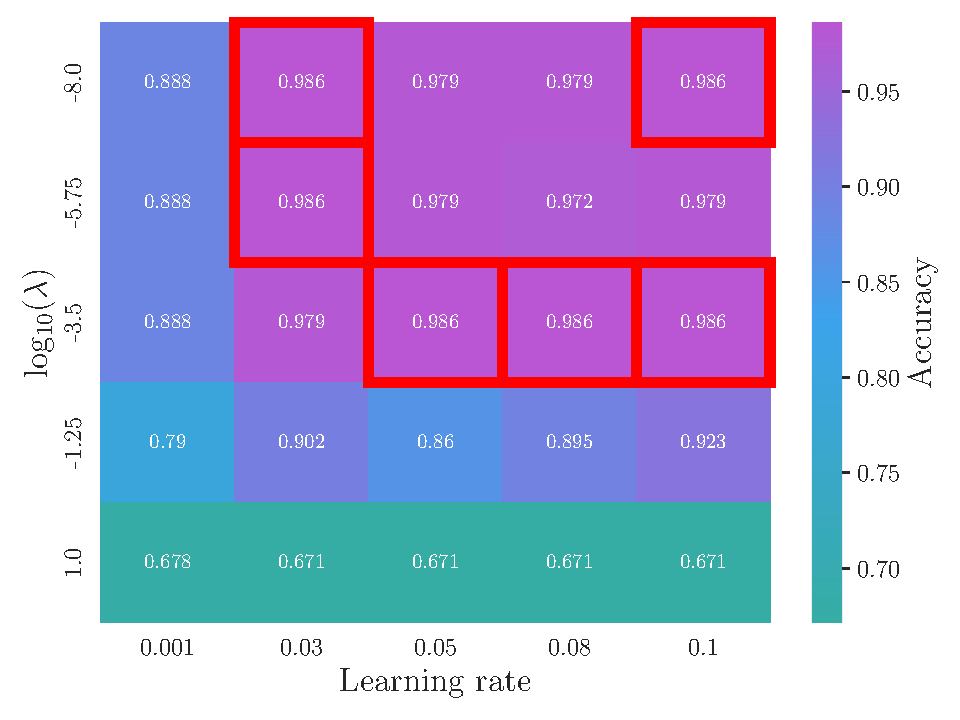
\includegraphics[width=\linewidth]{lmbda_lr_struct1_sigmoid.pdf}
                \caption{Network \network{2}{5} with a sigmoid activation function for the hidden layers. Multiple maxima was found with an accuracy of $0.993$.}
                \label[fig]{res:fig:clf_heatmap_N_2_5_sig}
            \end{subfigure}
            \hfill
            \begin{subfigure}{.49\textwidth}
                \centering
                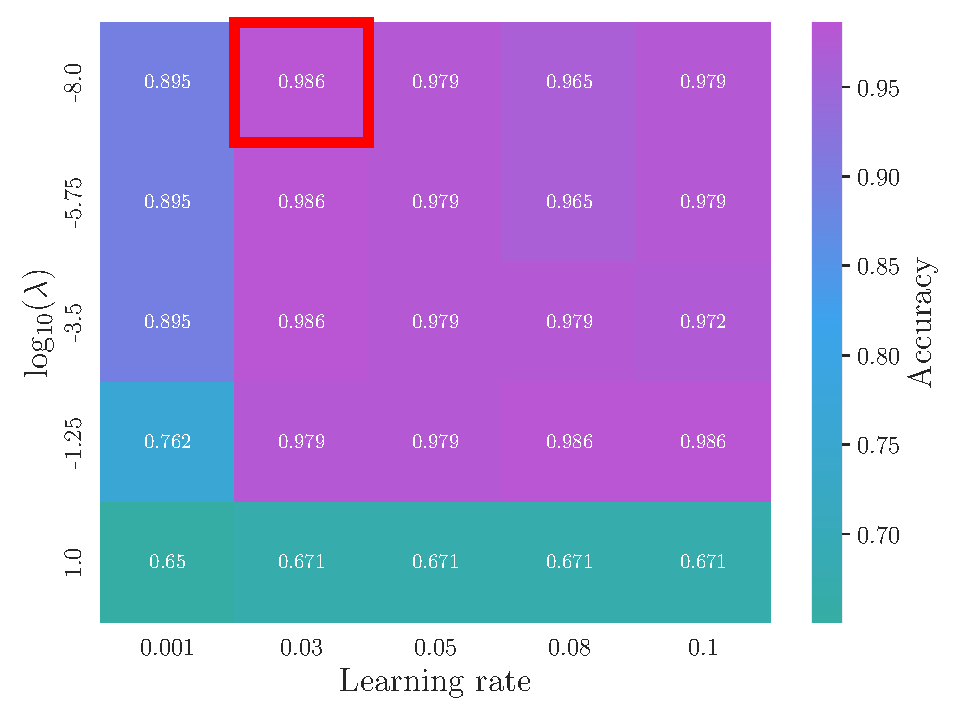
\includegraphics[width=\linewidth]{lmbda_lr_struct1_tanh.pdf}
                \caption{Network \network{2}{5} with a hyperbolic activation function for the hidden layers. A single maximum was found with accuracy of $0.993$, using $\eta = 0.03$ and $\lambda = 10^{-3.5}$}
                \label[fig]{res:fig:clf_heatmap_N_2_5_tanh}
            \end{subfigure}
            \caption{Plots of validation accuracy score varied against learning rate and penalisation term $\lambda$. Red squares mark the best accuracy scores. The first row contains the network structures \network{1}{5} with sigmoid (a) and hyperbolic tangent (b) activation functions for the output layer, while the second row contains \network{2}{5} with sigmoid (a) and hyperbolic tangent (b). The AdaGrad algorithm with momentum $\gamma = 0.8$ has been used for optimisation, running 100 epochs with a batch size of 200.}
            \label[fig]{res:fig:clf_heatmaps}
        \end{figure*}

        \begin{figure}
            \centering
            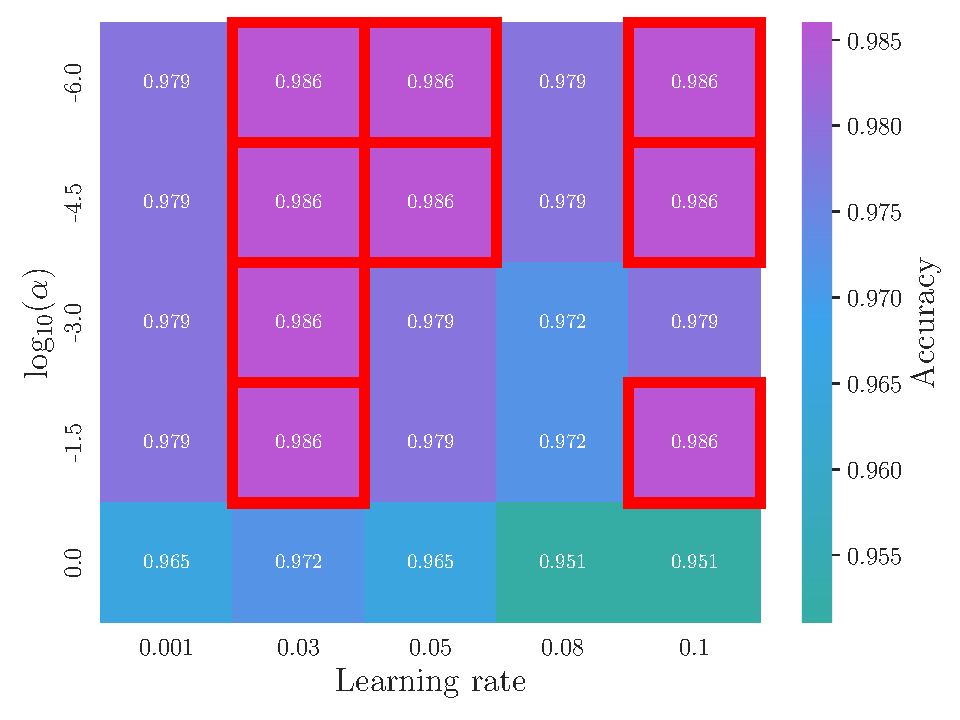
\includegraphics[width=\linewidth]{alpha_lr_struct1_sigmoid_sklearn.pdf}
            \caption
            {Network \network{2}{5} validation accuracy scores using SciKit-Learn's neural network implementation, varied against learning rate $\eta$ and $L_2$ penalisation term $\alpha$. Multiple maxima was found with an accuracy of 0.986.}
            \label[fig]{res:fig:clf_heatmap_sklearn}
        \end{figure}